\chapter{独立和与大数律}
\label{chap:laws-of-large-numbers}

掷一颗均匀骰子，点数的期望是$3.5$。掷$n$次后把点数平均，这个平均会不会越来越接近$3.5$？直觉说会，第~\ref{chap:random-variable-moments}章也正是用“多次重复的平均”来引出期望的。可是“接近”有两种不同的说法：对固定的$n$，平均偏离$3.5$超过$0.1$的概率很小；或者，几乎每一串实际掷出的点数，其平均最终都停在$3.5$附近。前一种只说每个时刻出错的机会，后一种说的是整条记录的最终走向。

另一个问题看起来不同。随机地给调和级数的每一项配上正负号，得到$\sum_k\varepsilon_k/k$，其中$\varepsilon_k$独立地以各$1/2$的概率取$\pm1$。不加符号时级数发散，加了随机符号以后，部分和会不会停下来？这里没有除以项数，问的是无限累计本身是否收敛。

两类问题有共同的对象：独立随机变量的部分和。平均是部分和除以$n$，级数是部分和本身。本章先计算部分和的均值与方差，并用Kolmogorov最大不等式控制部分和在一整段时间内的最大偏离；这一工具首先给出随机级数的收敛判据，再经截断推广为三系列定理。随后转向平均：弱大数律用方差或截断控制固定时刻的偏差概率，强大数律借Kronecker引理把加权级数的收敛翻译成平均的收敛。最后把频率、函数平均与样本矩写成独立同分布变量的平均，逐项核对条件。

全章使用第~\ref{chap:random-variable-convergence}章的几种收敛方式、Borel–Cantelli引理与支配收敛定理，独立性的一般含义取自第~\ref{chap:probability-spaces}章。

\section{独立部分和}
\label{sec:lln-partial-sums}

全章固定一个概率空间$(\Omega,\mathcal{F},\mathbb{P})$，在上面取一列随机变量$X_1,X_2,\dots$，并假设它们相互独立：其中任意有限个都相互独立。按第~\ref{chap:probability-spaces}章的结论，这些变量的函数，只要所用的下标组互不相交，也相互独立。例如$X_1+X_2$与$X_3X_4$独立，前$k$项的任何函数与第$k+1$项以后有限项的任何函数独立。

把前$n$项依次加起来，就得到一个随机的累计量。固定一个样本点$\omega$，$n\mapsto X_1(\omega)+\dots+X_n(\omega)$是一个普通的实数列，可以画成一条折线，每一步增加一个独立的增量。本章的所有问题都问这条折线的长期行为：它本身是否停在某处，或者除以步数以后是否停在某处。

\subsection{中心化与归一化}
\label{sec:lln-normalization}

同一列累计和可以按三种方式观察，它们回答的问题不同，先把记号定下来。

\begin{definition}[部分和、中心化部分和与样本平均]
\label{def:lln-partial-sums}
设$X_1,X_2,\dots$可积，记$\mu_k=\mathbb{E}[X_k]$。对$n\geq1$，令
\begin{equation}
 \begin{gathered}
 S_n=\sum_{k=1}^{n}X_k,\qquad \bar{X}_n=\frac{S_n}{n},\\
 \tilde{S}_n=\sum_{k=1}^{n}(X_k-\mu_k)=S_n-\mathbb{E}[S_n],
 \end{gathered}
 \label{eq:lln-partial-sums}
\end{equation}
并约定$S_0=\tilde{S}_0=0$。分别称$S_n$、$\tilde{S}_n$、$\bar{X}_n$为\term{部分和}（partial sum）、\term{中心化部分和}（centered partial sum）与\term{样本平均}（sample average）。
\end{definition}

$\mathbb{E}[S_n]=\sum_{k\leq n}\mu_k$用的是期望的线性性，下一小节再细看。部分和$S_n$收敛到有限极限，就是随机级数$\sum_kX_k$收敛，这是关于无限累计本身的问题。中心化部分和$\tilde{S}_n$去掉了各项的平均漂移，只剩随机波动；它是否收敛，问的是波动的累计能否停下来。样本平均$\bar{X}_n$把累计量按步数摊平，问的是每一步的平均贡献是否稳定。

\paragraph{同一列变量的不同答案}
取$X_k=\varepsilon_k$，其中$\varepsilon_1,\varepsilon_2,\dots$独立，各以$1/2$的概率取$+1$和$-1$。这样的$\varepsilon_k$称为随机符号，后文反复使用。这时$\mu_k=0$，三种部分和中前两种相同。$S_n$不可能收敛：相邻两项总相差$\lvert S_{n+1}-S_n\rvert=1$，对每个样本点都不是Cauchy列。平均$\bar{X}_n=S_n/n$却表现得很安稳。

图~\ref{fig:lln-three-normalizations}画出同一组五条路径的两种观察。图(a)中$S_n$在零的两侧来回游荡，偏离的典型大小与紫色虚线$\pm\sqrt{n}$同阶；图(b)中把同样的路径除以$n$，波动按$1/\sqrt{n}$收窄。下一小节会说明$\sqrt{n}$与$1/\sqrt{n}$分别是$S_n$与$\bar{X}_n$的标准差。

\begin{BookInlineFigure}
 \centering
 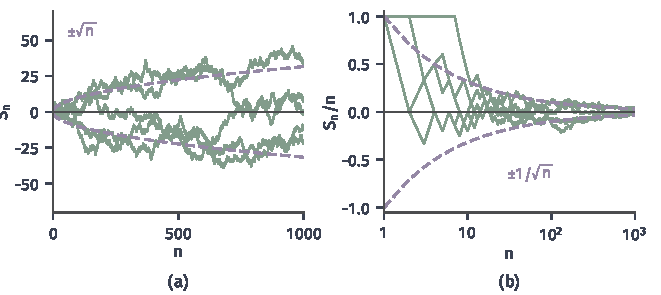
\includegraphics[width=112mm]{figures/07-probability/03-probability-limits/matplotlib/lln-three-normalizations/figure.pdf}
 \caption{随机符号的部分和与样本平均，五条路径（种子$7$）。(a)部分和$S_n$（绿线）与$\pm\sqrt{n}$（紫色虚线），横轴为线性刻度；(b)样本平均$S_n/n$（绿线）与$\pm1/\sqrt{n}$（紫色虚线），横轴为对数刻度。}
 \label{fig:lln-three-normalizations}
\end{BookInlineFigure}

反过来，给每一项加上递减的权重，累计也可能收敛。下一节将证明$\sum_k\varepsilon_k/k$几乎必然收敛，而$\sum_k\varepsilon_k/\sqrt{k}$几乎必然发散。级数问题与平均问题都由部分和出发，但所用的尺度不同，结论也就不同。

\paragraph{各项均值不同时}
当$X_k$不同分布时，各项均值$\mu_k$可以互不相同，中心化必须逐项减去自己的$\mu_k$。如果$\mu_k$的平均本身不收敛，就不存在一个共同的数可以作为$\bar{X}_n$的极限。

看一个具体的例子。令$X_k\sim\operatorname{Bern}(p_k)$相互独立，其中
\[
 p_k=\begin{cases}0.2, & 2^j\leq k<2^{j+1},\ j\ \text{为偶数},\\ 0.8, & 2^j\leq k<2^{j+1},\ j\ \text{为奇数}.\end{cases}
\]
第$j$段含$2^j$项，比前面所有段的项数之和还多一项，所以每走完一段，前$n$项均值的平均
\[
 m_n=\frac{1}{n}\sum_{k=1}^{n}p_k
\]
就被最后一段拉向它自己的取值。

具体算一下极限点。在第$J$段末尾$n=2^{J+1}-1$处，最后一段约占全部项数的$1/2$，倒数第二段约占$1/4$，依此类推。$J$为奇数时，取$0.8$的段占比约为$1/2+1/8+\dots=2/3$，于是
\[
 m_n\to0.8\cdot\tfrac23+0.2\cdot\tfrac13=0.6 ;
\]
$J$为偶数时两种取值的占比对调，$m_n\to0.4$。所以$m_n$在$0.4$与$0.6$之间往复，没有极限。

图~\ref{fig:lln-varying-means}(a)中蓝线是$m_n$，绿线是一条样本路径的$S_n/n$，后者紧跟前者摆动；图(b)画出两者之差$(S_n-\sum_{k\leq n}p_k)/n=\tilde{S}_n/n$，它趋于零。正确的问题因此是$\tilde{S}_n/n\to0$，而不是“$\bar{X}_n$趋于某个共同期望”。第~\ref{sec:lln-series-to-average}小节将证明，对这个例子$\tilde{S}_n/n$几乎必然趋于零。

\begin{BookInlineFigure}
 \centering
 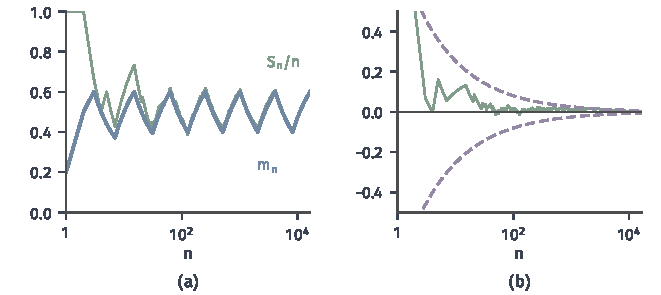
\includegraphics[width=112mm]{figures/07-probability/03-probability-limits/matplotlib/lln-varying-means/figure.pdf}
 \caption{分段取均值的独立Bernoulli变量，$p_k$在长度倍增的各段上交替取$0.2$与$0.8$，一条路径（种子$3$），横轴为对数刻度。(a)均值的平均$m_n$（蓝线）与样本平均$S_n/n$（绿线）；(b)差$(S_n-\sum_{k\leq n}p_k)/n$（绿线）与两倍标准差包络（紫色虚线）。}
 \label{fig:lln-varying-means}
\end{BookInlineFigure}

\subsection{均值与方差}
\label{sec:lln-mean-variance}

要判断累计量的走向，先看它在一个固定终点$n$处的中心和散布。中心由期望给出，不需要独立；散布由方差给出，独立性在这里第一次起作用。

\begin{theorem}[独立和的均值与方差]
\label{thm:lln-mean-variance}
设$X_1,\dots,X_n$可积，$\mu_k=\mathbb{E}[X_k]$。则
\begin{equation}
 \mathbb{E}[S_n]=\sum_{k=1}^{n}\mu_k .
 \label{eq:lln-sum-mean}
\end{equation}
若进一步$X_1,\dots,X_n$相互独立，且$\sigma_k^2=\operatorname{Var}(X_k)<\infty$，则
\begin{equation}
 \operatorname{Var}(S_n)=\mathbb{E}[\tilde{S}_n^2]=\sum_{k=1}^{n}\sigma_k^2 .
 \label{eq:lln-sum-variance}
\end{equation}
式~\eqref{eq:lln-sum-variance}只用到两两不相关，即$j\neq k$时$\operatorname{Cov}(X_j,X_k)=0$。
\end{theorem}

\begin{proof}
式~\eqref{eq:lln-sum-mean}是期望的线性性。对方差，记$D_k=X_k-\mu_k$，则$\tilde{S}_n=\sum_kD_k$。把平方展开成对角项与交叉项：
\[
 \tilde{S}_n^2=\sum_{k=1}^{n}D_k^2+\sum_{j\neq k}D_jD_k .
\]
由$\lvert D_jD_k\rvert\leq(D_j^2+D_k^2)/2$，每个交叉项都可积。$X_j$与$X_k$独立时，$D_j$与$D_k$也独立，乘积的期望等于期望的乘积，见第~\ref{chap:random-vectors}章，于是
\[
 \mathbb{E}[D_jD_k]=\mathbb{E}[D_j]\,\mathbb{E}[D_k]=0\cdot0=0 .
\]
对展开式取期望，交叉项全部消失，剩下$\sum_k\mathbb{E}[D_k^2]=\sum_k\sigma_k^2$。这一步只用了$\mathbb{E}[D_jD_k]=\operatorname{Cov}(X_j,X_k)=0$。
\end{proof}

\paragraph{波动为什么只按平方根增长}
把方差看作质量绕重心的转动惯量。独立的偏差有正有负，互相部分抵消，所以$n$项的总转动惯量只是各项之和，而不是像同向偏差那样按$n^2$增长。对比极端的相关情形：若$X_k=X_1$对所有$k$成立，则$S_n=nX_1$，方差为$n^2\sigma_1^2$。独立同分布、方差为$\sigma^2$时，式~\eqref{eq:lln-sum-variance}给出
\[
 \operatorname{Var}(S_n)=n\sigma^2,\qquad \operatorname{Var}(\bar{X}_n)=\frac{\sigma^2}{n} .
\]
部分和的标准差是$\sqrt{n}\,\sigma$，样本平均的标准差是$\sigma/\sqrt{n}$，这正是图~\ref{fig:lln-three-normalizations}中两条包络的来历。

\paragraph{固定终点的偏差}
对中心化部分和用第~\ref{chap:tail-probabilities}章的Chebyshev不等式，就得到终点处偏差的概率上界：对每个$a>0$，
\begin{equation}
 \mathbb{P}\bigl(\lvert\tilde{S}_n\rvert\geq a\bigr)\leq\frac{1}{a^2}\sum_{k=1}^{n}\sigma_k^2 .
 \label{eq:lln-endpoint-chebyshev}
\end{equation}

用骰子检验一下。掷$n=100$次均匀骰子，单次点数的方差为$35/12$，所以
\[
 \operatorname{Var}(S_{100})=100\cdot\frac{35}{12}=\frac{875}{3}\approx291.7 .
\]
取$a=30$，式~\eqref{eq:lln-endpoint-chebyshev}给出
\[
 \mathbb{P}\bigl(\lvert S_{100}-350\rvert\geq30\bigr)\leq\frac{291.7}{900}\approx0.324 .
\]
用$200000$条模拟路径（种子$12$）估计，左边约为$0.085$。界偏大，但它对任何方差为$35/12$的独立同分布序列都成立。

\paragraph{终点控制不住整段路径}
式~\eqref{eq:lln-endpoint-chebyshev}只管时刻$n$。部分和可以先越过$\pm a$，再回到区间内部。图~\ref{fig:lln-endpoint-vs-path}画出$30$条骰子路径（种子$11$），其中$4$条在$k\leq100$的某一步越过了$\pm30$，有$3$条到$k=100$时又回到了带内。模拟估计全程越过的概率约为$0.147$，比终点越过的$0.085$大不少。

\begin{BookInlineFigure}
 \centering
 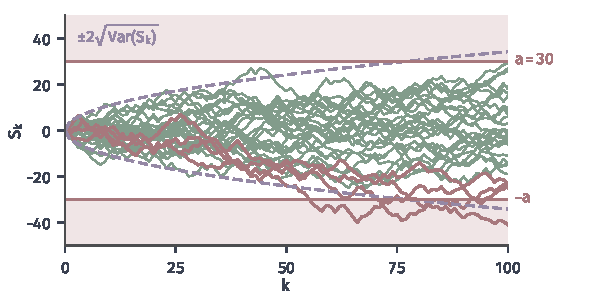
\includegraphics[width=100mm]{figures/07-probability/03-probability-limits/matplotlib/lln-endpoint-vs-path/figure.pdf}
 \caption{中心化骰子部分和$S_k=\sum_{i\leq k}(D_i-3.5)$的$30$条路径（种子$11$），$k\leq100$。红色水平线为阈值$\pm30$，浅红区域为越界区域；红线是在某一步越过阈值的路径，绿线是始终未越过的路径；紫色虚线为$\pm2\sqrt{\operatorname{Var}(S_k)}$。}
 \label{fig:lln-endpoint-vs-path}
\end{BookInlineFigure}

一个朴素的补救是对每个$k\leq n$分别用Chebyshev不等式再相加。独立同分布、方差为$\sigma^2$时，
\[
 \mathbb{P}\Bigl(\max_{k\leq n}\lvert\tilde{S}_k\rvert\geq a\Bigr)\leq\sum_{k=1}^{n}\frac{\operatorname{Var}(S_k)}{a^2}=\frac{\sigma^2}{a^2}\cdot\frac{n(n+1)}{2} .
\]
骰子例子中右边约为$16.4$，远大于$1$，毫无用处。各个时刻的越界事件高度重叠，相加把同一块概率计算了许多次。下一小节说明，对独立中心化的和，整段路径的最大偏离与终点偏差满足同一个上界。

\subsection{Kolmogorov最大不等式}
\label{sec:lln-maximal-inequality}

先猜一下最大偏离应当满足怎样的界。一条路径若在某一步$k$首次越过$a$，此后的增量既独立于过去，平均又为零，没有系统地把路径拉回来的倾向。所以终点平方的期望至少还保留着越界时的$S_k^2\geq a^2$。这就是说，越过阈值的路径不会因为“回头”而在终点的方差中消失。

\begin{theorem}[Kolmogorov最大不等式]
\label{thm:lln-kolmogorov-maximal}
设$X_1,\dots,X_n$相互独立，$\mathbb{E}[X_k]=0$，$\mathbb{E}[X_k^2]<\infty$。则对每个$a>0$，
\begin{equation}
 \mathbb{P}\Bigl(\max_{1\leq k\leq n}\lvert S_k\rvert\geq a\Bigr)\leq\frac{\operatorname{Var}(S_n)}{a^2}=\frac{1}{a^2}\sum_{k=1}^{n}\mathbb{E}[X_k^2] .
 \label{eq:lln-kolmogorov-maximal}
\end{equation}
\end{theorem}

这个不等式称为\term{Kolmogorov最大不等式}（Kolmogorov's maximal inequality）。它的右边与终点的Chebyshev界~\eqref{eq:lln-endpoint-chebyshev}完全相同，左边却换成了整段路径的最大值。

\begin{proof}
按首次越过阈值的时刻把事件拆开。对$k=1,\dots,n$，令
\[
 A_k=\bigl\{\lvert S_k\rvert\geq a,\ \lvert S_j\rvert<a\ \text{对所有}\ j<k\bigr\} .
\]
$A_k$表示“在第$k$步首次越过”。这些事件两两不交，它们的并恰为$A=\{\max_{k\leq n}\lvert S_k\rvert\geq a\}$。

由于$S_n^2\geq0$，且$A_1,\dots,A_n$不交，
\[
 \mathbb{E}[S_n^2]\geq\mathbb{E}[S_n^2\mathbf{1}_{A}]=\sum_{k=1}^{n}\mathbb{E}[S_n^2\mathbf{1}_{A_k}] .
\]
固定$k$，把终点写成首次越过时的位置加上之后的增量，$S_n=S_k+(S_n-S_k)$。展开平方并丢掉非负项$(S_n-S_k)^2$，得到
\[
 S_n^2\geq S_k^2+2S_k(S_n-S_k) .
\]

关键是交叉项的期望为零。$S_k\mathbf{1}_{A_k}$只依赖$X_1,\dots,X_k$，$S_n-S_k=X_{k+1}+\dots+X_n$只依赖后面的变量，两者独立，并且都平方可积。于是
\[
 \mathbb{E}\bigl[S_k\mathbf{1}_{A_k}(S_n-S_k)\bigr]=\mathbb{E}[S_k\mathbf{1}_{A_k}]\,\mathbb{E}[S_n-S_k]=0 .
\]

把上面的不等式乘以$\mathbf{1}_{A_k}$再取期望，交叉项消失。再利用$A_k$上$S_k^2\geq a^2$，得到
\[
 \mathbb{E}[S_n^2\mathbf{1}_{A_k}]\geq\mathbb{E}[S_k^2\mathbf{1}_{A_k}]\geq a^2\,\mathbb{P}(A_k) .
\]
对$k$求和，并利用$A_1,\dots,A_n$不交，得到
\[
 \mathbb{E}[S_n^2]\geq a^2\sum_{k=1}^{n}\mathbb{P}(A_k)=a^2\,\mathbb{P}(A) .
\]
最后由式~\eqref{eq:lln-sum-variance}，左边等于$\operatorname{Var}(S_n)=\sum_k\mathbb{E}[X_k^2]$，两边除以$a^2$即得。
\end{proof}

图~\ref{fig:lln-first-passage}把证明中的分解画了出来。首次越过时刻$k$之前的信息决定了$A_k$与$S_k$，之后的增量与它们独立且平均为零。路径越界后可能回到带内，但这种回头只是随机的，平均来说不抵消越界时已有的$S_k^2$。

\begin{BookInlineFigure}
 \centering
 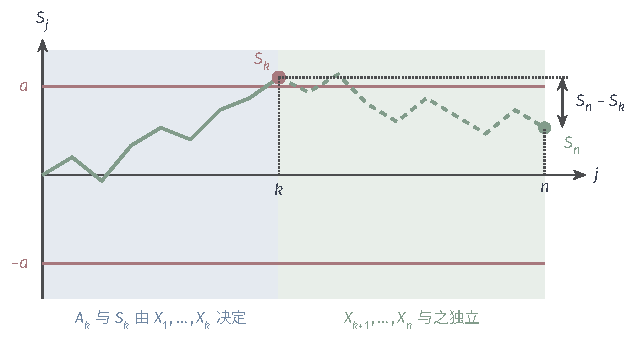
\includegraphics[width=107mm]{figures/07-probability/03-probability-limits/tikz/lln-first-passage/figure.pdf}
 \caption{Kolmogorov最大不等式的首次越过分解（示意）。绿色折线为部分和路径，在第$k$步首次达到$\lvert S_k\rvert\geq a$（红点）；浅蓝区域内的信息决定事件$A_k$，浅绿区域内的增量$X_{k+1},\dots,X_n$与之独立；终点$S_n=S_k+(S_n-S_k)$可以回到阈值以内。}
 \label{fig:lln-first-passage}
\end{BookInlineFigure}

\paragraph{一个能逐条数清的例子}
取四个随机符号，$S_k=\varepsilon_1+\dots+\varepsilon_k$，共有$2^4=16$条等可能的路径，阈值取$a=3$。图~\ref{fig:lln-rademacher-lattice}在每个节点标出经过它的路径条数。要在四步内达到$\lvert S_k\rvert\geq3$，必须前三步同号，到达$(3,\pm3)$；从那里第四步可上可下，所以共有$2\times2=4$条路径越界。终点满足$\lvert S_4\rvert\geq3$的只有终点为$\pm4$的$2$条。

\begin{BookInlineFigure}
 \centering
 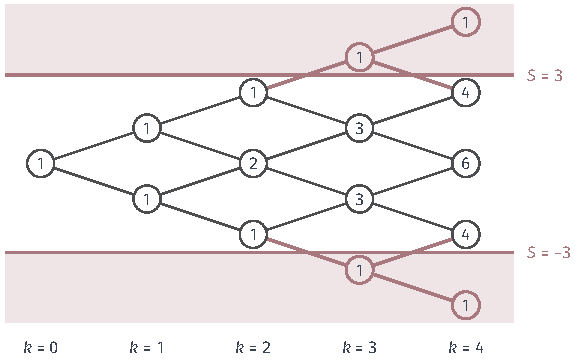
\includegraphics[width=98mm]{figures/07-probability/03-probability-limits/tikz/lln-rademacher-lattice/figure.pdf}
 \caption{四个随机符号的全部$16$条路径。节点中的数字是经过该节点的路径条数；红色水平线为$S=\pm3$，红色边与红框节点标出在某一步达到$\lvert S_k\rvert\geq3$的$4$条路径，其中$2$条在第四步回到$\pm2$。}
 \label{fig:lln-rademacher-lattice}
\end{BookInlineFigure}

于是三个量分别是
\[
 \begin{gathered}
 \mathbb{P}\Bigl(\max_{k\leq4}\lvert S_k\rvert\geq3\Bigr)=\frac{4}{16}=0.25,\qquad
 \mathbb{P}(\lvert S_4\rvert\geq3)=\frac{2}{16}=0.125,\\
 \frac{\operatorname{Var}(S_4)}{3^2}=\frac49\approx0.444 .
 \end{gathered}
\]
最大偏离的概率是终点概率的两倍，仍在Kolmogorov界之下。若取$a=2$，同样计数得到$0.75$、$0.625$与界$1$。

\paragraph{较长的路径}
图~\ref{fig:lln-maximal-compare}对$n=100$个随机符号精确计算两种概率：终点概率由二项分布求和，全程最大值越界的概率由逐步递推（越界即吸收）求得。$a=20$时终点概率为$0.057$，全程概率为$0.092$，Kolmogorov界为$0.25$，逐点相加的界却是$12.6$。Kolmogorov界与真实值的差距来自它只用了方差；真正的尾部还要轻得多，那是第~\ref{chap:central-limit-theorem}章的内容。

\begin{BookInlineFigure}
 \centering
 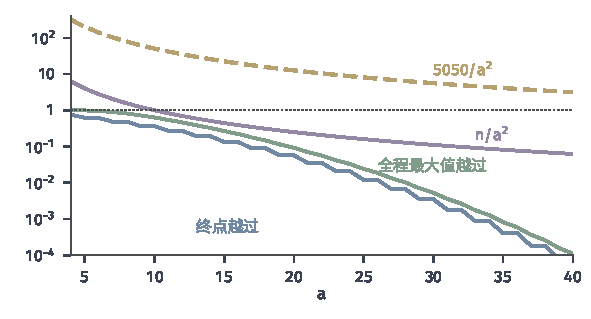
\includegraphics[width=100mm]{figures/07-probability/03-probability-limits/matplotlib/lln-maximal-compare/figure.pdf}
 \caption{$n=100$个随机符号，越界概率随阈值$a$的变化，纵轴为对数刻度。蓝线为终点概率$\mathbb{P}(\lvert S_n\rvert\geq a)$，绿线为全程最大值概率$\mathbb{P}(\max_{k\leq n}\lvert S_k\rvert\geq a)$，二者均为精确值；紫线为Kolmogorov界$n/a^2$，黄色虚线为逐点相加的界$\sum_{k\leq n}k/a^2=5050/a^2$，点线标出概率$1$。}
 \label{fig:lln-maximal-compare}
\end{BookInlineFigure}

\paragraph{条件各起什么作用}
中心化不可省略。若$X_k\equiv1$，方差为零，式~\eqref{eq:lln-kolmogorov-maximal}右边为$0$，而$\max_{k\leq n}\lvert S_k\rvert=n$。证明中用到的是$\mathbb{E}[S_n-S_k]=0$：有漂移时，越界之后的路径会被系统地推向一侧，平方的期望不再只由方差决定。

独立性也不可省略，它保证了交叉项的期望为零。取$X_1=\varepsilon_1$，$X_2=-\varepsilon_1$，两项都中心化且方差为$1$，但$S_2=0$，右边为$0$；左边在$a=1$时却等于$\mathbb{P}(\lvert S_1\rvert\geq1)=1$。这里第二步完全由第一步决定，越界后被确定地拉了回来。

这个不等式是本章的主要工具。下一节用它控制随机级数的尾段，第~\ref{sec:lln-strong-law}节再经由级数得到强大数律。


\section{独立随机级数}
\label{sec:lln-random-series}

回到章首的随机调和级数$\sum_k\varepsilon_k/k$。确定的调和级数$\sum_k1/k$发散，是因为每一项都向同一方向推；随机符号让各项方向随机，推力互相抵消。抵消到什么程度，部分和才会停下来？

一般地，设$X_1,X_2,\dots$独立，问部分和$S_n=\sum_{k\leq n}X_k$是否几乎必然收敛到一个有限的极限$S$。这样的$\sum_kX_k$称为\term{随机级数}（random series）。对每个样本点$\omega$，这是一个普通的数项级数，收敛与否由Cauchy准则判断：
\[
 S_n(\omega)\ \text{收敛}\iff \sup_{j,k>m}\lvert S_j(\omega)-S_k(\omega)\rvert\to0\quad(m\to\infty) .
\]
上确界只需在可数个下标上取，所以“级数收敛”是一个事件。我们要证明的是这个事件的概率为一。

图~\ref{fig:lln-random-harmonic}用同一组随机符号画出两个级数的部分和。图(a)中$\sum_k\varepsilon_k/k$的六条路径在$n=100$以后几乎不再移动，各自停在不同的高度；图(b)中$\sum_k\varepsilon_k/\sqrt{k}$的路径一直在游荡，摆幅与紫色包络$\pm2\sqrt{H_n}$同步扩大，其中$H_n=\sum_{k\leq n}1/k$。两者的区别正在于各项方差之和：前者$\sum_k1/k^2<\infty$，后者$\sum_k1/k=\infty$。

\begin{BookInlineFigure}
 \centering
 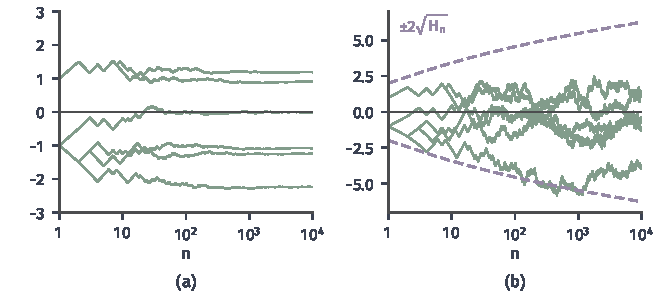
\includegraphics[width=112mm]{figures/07-probability/03-probability-limits/matplotlib/lln-random-harmonic/figure.pdf}
 \caption{同一组随机符号（种子$5$）下两个随机级数的部分和，六条路径，横轴为对数刻度。(a)$\sum_{k\leq n}\varepsilon_k/k$；(b)$\sum_{k\leq n}\varepsilon_k/\sqrt{k}$，紫色虚线为$\pm2\sqrt{H_n}$，$H_n=\sum_{k\leq n}1/k$。}
 \label{fig:lln-random-harmonic}
\end{BookInlineFigure}

\subsection{方差可和的情形}
\label{sec:lln-variance-series}

收敛需要控制部分和的整个尾段，而不仅是某一个时刻的增量。Kolmogorov最大不等式恰好控制一整段路径的最大偏离，把它用在从第$m+1$项开始的尾段上，偏离的概率由尾段方差之和决定。方差可和时，这个尾和趋于零。

\begin{theorem}[方差可和的随机级数]
\label{thm:lln-variance-series}
设$X_1,X_2,\dots$相互独立，$\mathbb{E}[X_k]=0$，并且
\begin{equation}
 \sum_{k=1}^{\infty}\mathbb{E}[X_k^2]<\infty .
 \label{eq:lln-variance-summable}
\end{equation}
则$\sum_kX_k$几乎必然收敛到一个有限的随机变量$S$。此外$S_n\xrightarrow{L^{2}}S$，并且$\mathbb{E}[S]=0$，$\mathbb{E}[S^2]=\sum_k\mathbb{E}[X_k^2]$。
\end{theorem}

\begin{proof}
记$\sigma_k^2=\mathbb{E}[X_k^2]$。对$m\geq0$，令
\[
 V_m=\sup_{j,k>m}\lvert S_j-S_k\rvert,\qquad W_m=\sup_{k>m}\lvert S_k-S_m\rvert ,
\]
二者取值于$[0,\infty]$。$V_m$随$m$不增，所以极限$V=\lim_mV_m$存在，并且部分和是Cauchy列当且仅当$V=0$。对$j,k>m$用三角不等式，
\[
 \lvert S_j-S_k\rvert\leq\lvert S_j-S_m\rvert+\lvert S_k-S_m\rvert\leq2W_m ,
\]
所以$V_m\leq2W_m$。

先估计$W_m$。固定$m$与$\varepsilon>0$，对$N>m$考虑事件
\[
 E_N=\Bigl\{\max_{m<k\leq N}\lvert S_k-S_m\rvert>\varepsilon\Bigr\} .
\]
$E_N$随$N$增大而增大，并上升到$\{W_m>\varepsilon\}$。尾段$S_k-S_m=X_{m+1}+\dots+X_k$是独立中心化变量的部分和，对它用定理~\ref{thm:lln-kolmogorov-maximal}，得到
\[
 \mathbb{P}(E_N)\leq\frac{1}{\varepsilon^2}\sum_{k=m+1}^{N}\sigma_k^2\leq\frac{1}{\varepsilon^2}\sum_{k>m}\sigma_k^2 .
\]
令$N\to\infty$，由概率的连续性，
\begin{equation}
 \mathbb{P}(W_m>\varepsilon)\leq\frac{1}{\varepsilon^2}\sum_{k>m}\sigma_k^2 .
 \label{eq:lln-tail-oscillation}
\end{equation}

再回到$V$。由于$V\leq V_m\leq2W_m$，对每个$m$，
\[
 \mathbb{P}(V>2\varepsilon)\leq\mathbb{P}(W_m>\varepsilon)\leq\frac{1}{\varepsilon^2}\sum_{k>m}\sigma_k^2 .
\]
左边与$m$无关，右边是收敛级数~\eqref{eq:lln-variance-summable}的尾和，令$m\to\infty$趋于零。所以对每个$\varepsilon>0$都有$\mathbb{P}(V>2\varepsilon)=0$。取$\varepsilon=1/j$并对$j$取可数并，得到$\mathbb{P}(V>0)=0$。于是几乎必然地，$S_n$是Cauchy列，收敛到有限极限$S$。

最后看$L^2$收敛。由式~\eqref{eq:lln-sum-variance}，$N>m$时
\[
 \mathbb{E}\bigl[(S_N-S_m)^2\bigr]=\sum_{k=m+1}^{N}\sigma_k^2\leq\sum_{k>m}\sigma_k^2\to0 .
\]
所以$S_n$在$L^2$中是Cauchy列，收敛到某个$S'\in L^2$。由第~\ref{chap:random-variable-convergence}章，$L^2$收敛的序列有几乎必然收敛的子列，其极限只能是$S$，故$S'=S$几乎必然成立。$L^2$收敛蕴含一阶矩与二阶矩收敛，于是
\[
 \mathbb{E}[S]=\lim_{n\to\infty}\mathbb{E}[S_n]=0,\qquad \mathbb{E}[S^2]=\lim_{n\to\infty}\mathbb{E}[S_n^2]=\sum_k\sigma_k^2 .
\]
\end{proof}

证明的结构值得记住：几乎必然收敛归结为“尾段的最大振荡依概率趋于零”，而最大振荡正是Kolmogorov不等式所控制的量。只控制单个增量$S_N-S_m$的方差，只能得到$L^2$收敛，不足以说明每条路径都停下来。

\paragraph{随机调和级数}
对$X_k=\varepsilon_k/k$，各项均值为零，方差可和：
\[
 \mathbb{E}[X_k]=0,\qquad \sum_{k=1}^{\infty}\mathbb{E}[X_k^2]=\sum_{k=1}^{\infty}\frac{1}{k^2}=\frac{\pi^2}{6} .
\]
定理~\ref{thm:lln-variance-series}给出$\sum_k\varepsilon_k/k$几乎必然收敛，极限$S$的均值为$0$，方差为$\pi^2/6\approx1.645$。尾和满足$\sum_{k>m}1/k^2<1/m$，取$\varepsilon=1/4$与$m=100$，式~\eqref{eq:lln-tail-oscillation}给出
\[
 \mathbb{P}\Bigl(\sup_{k>100}\lvert S_k-S_{100}\rvert>\tfrac14\Bigr)\leq16\sum_{k>100}\frac{1}{k^2}\approx16\times0.00995\approx0.159 .
\]

图~\ref{fig:lln-harmonic-limit}(b)把这个界与模拟频率放在一起比较（$4000$条路径，种子$8$，上确界在$k\leq20000$内计算）。$m=100$时模拟频率约为$0.028$。两条曲线都随$m$按$1/m$的阶下降，界比真实值宽松，但单凭方差就保证了尾段的振荡越来越罕见。

\begin{BookInlineFigure}
 \centering
 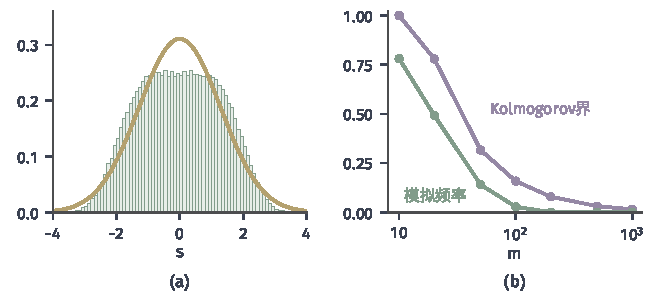
\includegraphics[width=112mm]{figures/07-probability/03-probability-limits/matplotlib/lln-harmonic-limit/figure.pdf}
 \caption{随机调和级数$\sum_k\varepsilon_k/k$的极限与尾段振荡。(a)$S_{1000}$的直方图（浅绿，$200000$个样本，种子$2$）与方差相同的高斯密度$\mathcal{N}(0,\pi^2/6)$（黄线）；(b)尾段最大振荡$\max_{m<k\leq20000}\lvert S_k-S_m\rvert\geq1/4$的模拟频率（绿线，$4000$条路径，种子$8$）与Kolmogorov界$16\sum_{m<k\leq20000}1/k^2$（紫线），横轴为$m$的对数刻度。}
 \label{fig:lln-harmonic-limit}
\end{BookInlineFigure}

极限$S$是一个真正的随机变量，它的分布由全部项共同决定。图~\ref{fig:lln-harmonic-limit}(a)用$S_{1000}$代替$S$，二者之差的方差$\sum_{k>1000}1/k^2$小于$10^{-3}$。直方图顶部平坦，与同方差的高斯密度明显不同。用独立性展开四次方可以核对这一点：对$S_n=\sum_{k\leq n}a_k\varepsilon_k$，奇次项的期望为零，只剩每个下标出现偶数次的项，
\[
 \mathbb{E}[S_n^4]=\sum_{k}a_k^4+3\sum_{j\neq k}a_j^2a_k^2=3\Bigl(\sum_ka_k^2\Bigr)^2-2\sum_ka_k^4 .
\]
取$a_k=1/k$并令$n\to\infty$，用$\sum_k1/k^4=\pi^4/90$，得到
\[
 \frac{\mathbb{E}[S^4]}{(\mathbb{E}[S^2])^2}-3=-\frac{2\pi^4/90}{(\pi^2/6)^2}=-0.8 ,
\]
而高斯分布的这个值为$0$。模拟值约为$-0.81$。

\paragraph{中心化不可省略}
定理要求各项均值为零。若$X_k=1/k$是确定的常数，方差全为零，条件~\eqref{eq:lln-variance-summable}成立，级数却发散。一般地，若$\sum_k\operatorname{Var}(X_k)<\infty$，对$X_k-\mu_k$用定理~\ref{thm:lln-variance-series}，得到$\sum_k(X_k-\mu_k)$几乎必然收敛。两个级数之差是数项级数$\sum_k\mu_k$，所以
\[
 \sum_kX_k\ \text{几乎必然收敛}\iff\sum_k\mu_k\ \text{收敛} ,
\]
并且$\sum_k\mu_k$发散时$\sum_kX_k$几乎必然发散。例如取$X_k=\xi_k/k$，$\xi_k\sim\operatorname{Bern}(1/2)$独立，方差$1/(4k^2)$可和，但均值$1/(2k)$的级数发散，于是$\sum_kX_k=+\infty$几乎必然成立。方差控制随机波动，均值控制系统漂移，两件事要分别检查。

\subsection{截断与大项控制}
\label{sec:lln-truncation}

方差可和是充分条件，但不是必要条件。各项可能偶尔取极大的值，使方差甚至均值都很大或无穷，而这些大值只出现有限次，对级数是否收敛没有影响。

\paragraph{一个方差与均值都失效的例子}
令$X_1=\varepsilon_1$。对$k\geq2$，取与$\varepsilon_k$独立的事件$B_k$，$\mathbb{P}(B_k)=1/k^2$，各$B_k$与各$\varepsilon_k$全体相互独立，定义
\[
 X_k=\begin{cases}k, & B_k\ \text{发生},\\ \varepsilon_k/k, & B_k\ \text{不发生}.\end{cases}
\]
大值$k$出现的机会很小，但幅度很大。逐项计算，$k\geq2$时
\[
 \mathbb{E}[X_k]=k\cdot\frac{1}{k^2}=\frac1k,\qquad
 \operatorname{Var}(X_k)=1+\frac{1}{k^2}-\frac{1}{k^4}-\frac{1}{k^2}=1-\frac{1}{k^4} .
\]
这里用了$\mathbb{E}[X_k^2]=k^2/k^2+(1-1/k^2)/k^2$。方差之和与均值之和都发散，上一小节的判据完全用不上。

然而大项出现的概率可和：
\[
 \sum_{k\geq2}\mathbb{P}(B_k)=\frac{\pi^2}{6}-1\approx0.645<\infty .
\]
由第~\ref{chap:random-variable-convergence}章的Borel–Cantelli引理，几乎必然只有有限个$B_k$发生。对这样的样本点，从某一项起$X_k=\varepsilon_k/k$，而$\sum_k\varepsilon_k/k$几乎必然收敛，改动有限项不影响收敛。所以$\sum_kX_k$几乎必然收敛。

图~\ref{fig:lln-big-terms}画出六条路径（种子$4$）。其中三条各出现一次大项（红点，分别在$k=2,10,2$处），路径随之跳起，此后与其余路径一样停住。黄色虚线是各项期望的累计$\sum_{k\leq n}\mathbb{E}[X_k]$，按$\ln n$无限增长：期望被极少发生的大值撑大，它描述的不是典型路径。

\begin{BookInlineFigure}
 \centering
 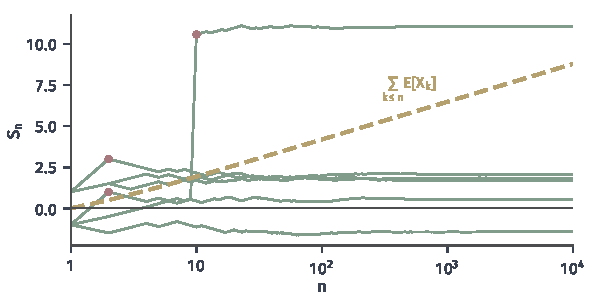
\includegraphics[width=100mm]{figures/07-probability/03-probability-limits/matplotlib/lln-big-terms/figure.pdf}
 \caption{含罕见大项的随机级数，六条路径（种子$4$），横轴为对数刻度。绿线为部分和$S_n$，红点标出大项$X_k=k$出现的位置；黄色虚线为期望的累计$\sum_{k\leq n}\mathbb{E}[X_k]=\sum_{2\leq k\leq n}1/k$。}
 \label{fig:lln-big-terms}
\end{BookInlineFigure}

\paragraph{一般的截断}
这个例子的做法可以一般化：先把大值切掉，再对剩下的有界部分分别处理均值与波动。固定$c>0$，令
\begin{equation}
 Y_k=X_k\mathbf{1}_{\{\lvert X_k\rvert\leq c\}} .
 \label{eq:lln-truncation}
\end{equation}
称$Y_k$为$X_k$在水平$c$处的\term{截断}（truncation）。每一项因此拆成三部分：
\[
 X_k=\bigl(X_k-Y_k\bigr)+\mathbb{E}[Y_k]+\bigl(Y_k-\mathbb{E}[Y_k]\bigr) .
\]
第一部分只在$\lvert X_k\rvert>c$时非零，是大项；第二部分是截断后的均值，一个普通的数；第三部分是有界的中心化波动。

三部分各需要一种控制，图~\ref{fig:lln-truncation-split}画出这种分工。

\begin{BookInlineFigure}
 \centering
 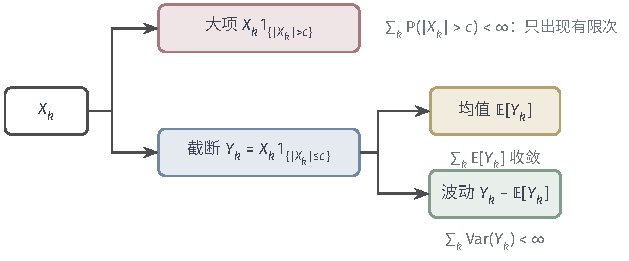
\includegraphics[width=106mm]{figures/07-probability/03-probability-limits/tikz/lln-truncation-split/figure.pdf}
 \caption{在固定水平$c$截断后的三部分及各自的控制条件。浅红框为大项，由超阈值概率之和控制；浅黄框为截断均值，由数项级数控制；浅绿框为中心化波动，由截断方差之和控制。}
 \label{fig:lln-truncation-split}
\end{BookInlineFigure}

\begin{enumerate}
 \item \emph{大项只出现有限次。}若$\sum_k\mathbb{P}(\lvert X_k\rvert>c)<\infty$，由Borel–Cantelli引理，几乎必然存在$N(\omega)$，使$k>N(\omega)$时$X_k(\omega)=Y_k(\omega)$。于是$n>N(\omega)$时$S_n(\omega)-\sum_{k\leq n}Y_k(\omega)$是一个不再变化的有限数，$\sum_kX_k$与$\sum_kY_k$同时收敛或同时发散。这一步不需要独立性，也不要求$X_k$有任何矩。
 \item \emph{截断均值的级数收敛。}$\lvert Y_k\rvert\leq c$，所以$\mathbb{E}[Y_k]$总存在。$\sum_k\mathbb{E}[Y_k]$是一个数项级数，它收敛与否与随机性无关，只能直接检查。
 \item \emph{截断波动的方差可和。}$Y_k-\mathbb{E}[Y_k]$是独立变量$X_k$的函数，彼此独立，均值为零，绝对值不超过$2c$。若$\sum_k\operatorname{Var}(Y_k)<\infty$，由定理~\ref{thm:lln-variance-series}，$\sum_k(Y_k-\mathbb{E}[Y_k])$几乎必然收敛。
\end{enumerate}

三种控制各管一件事。第一种处理方差无法描述的重尾大值；第二种处理系统性漂移；第三种处理有界的随机波动。截断水平$c$固定不变，有界性使第三步可以只用方差。回到上面的例子，取$c=1$：$k\geq2$时$\lvert X_k\rvert>1$恰好是$B_k$发生，$Y_k=\varepsilon_k\mathbf{1}_{B_k^{\mathrm{c}}}/k$，均值为$0$，方差$(1-1/k^2)/k^2$可和，三项都满足。

\subsection{三系列定理}
\label{sec:lln-three-series}

把上一小节的三种控制合在一起，就得到一个随机级数几乎必然收敛的充分条件。Kolmogorov证明了这三个条件也是必要的。

\begin{theorem}[三系列定理]
\label{thm:lln-three-series}
设$X_1,X_2,\dots$相互独立，$c>0$，$Y_k=X_k\mathbf{1}_{\{\lvert X_k\rvert\leq c\}}$。则$\sum_kX_k$几乎必然收敛，当且仅当下面三个级数都收敛：
\begin{equation}
 \sum_{k}\mathbb{P}(\lvert X_k\rvert>c),\qquad
 \sum_{k}\mathbb{E}[Y_k],\qquad
 \sum_{k}\operatorname{Var}(Y_k) .
 \label{eq:lln-three-series}
\end{equation}
\end{theorem}

这一结论称为\term{三系列定理}（three-series theorem）。注意第二个级数只要求收敛，不要求绝对收敛。例如确定的$X_k=(-1)^k/k$，取$c=1$时$Y_k=X_k$，第一、三个级数为零，第二个是条件收敛的交错级数，$\sum_kX_k$确实收敛。

\begin{proof}[充分性的证明]
设三个级数都收敛。由第三个级数与定理~\ref{thm:lln-variance-series}，$\sum_k(Y_k-\mathbb{E}[Y_k])$几乎必然收敛；加上收敛的数项级数$\sum_k\mathbb{E}[Y_k]$，$\sum_kY_k$几乎必然收敛。由第一个级数与Borel–Cantelli引理，几乎必然只有有限个$k$使$X_k\neq Y_k$，所以$\sum_kX_k$与$\sum_kY_k$同时收敛。两个几乎必然事件的交仍是几乎必然事件，结论成立。
\end{proof}

必要性中，第一个级数的必要性可以直接证明。若$\sum_kX_k$几乎必然收敛，则$X_k\to0$几乎必然，所以$\lvert X_k\rvert>c$几乎必然只发生有限次。事件$\{\lvert X_k\rvert>c\}$相互独立；如果$\sum_k\mathbb{P}(\lvert X_k\rvert>c)=\infty$，Borel–Cantelli引理的第二部分会给出它们几乎必然发生无穷多次，矛盾。

另两个级数的必要性需要更细的估计，篇幅较长，读者可查阅~\scite{math-kallenberg2021probability}。其机制是：若截断方差之和发散，有界独立波动的累计会像标准差$\sqrt{\sum_{k\leq n}\operatorname{Var}(Y_k)}$那样不断扩大，不可能停在一处，这与图~\ref{fig:lln-random-harmonic}(b)的情形相同；方差可和而均值级数发散时，前面已经说明级数几乎必然发散。同一参考书还说明，独立随机级数收敛的概率只能是$0$或$1$，所以三个级数中只要有一个发散，$\sum_kX_k$就几乎必然发散。

\paragraph{截断水平的选择}
定理对每个固定的$c>0$都成立。由必要性，若三个级数对某个$c$都收敛，则级数收敛，从而它们对所有$c>0$都收敛。实际使用时取最方便的$c$即可。

\paragraph{随机符号级数}
设$(a_k)$是有界实数列，考虑$\sum_ka_k\varepsilon_k$。取$c>\sup_k\lvert a_k\rvert$，截断不改变任何一项：第一个级数为零，$\mathbb{E}[Y_k]=0$，$\operatorname{Var}(Y_k)=a_k^2$。由三系列定理，
\begin{equation}
 \sum_ka_k\varepsilon_k\ \text{几乎必然收敛}\iff\sum_ka_k^2<\infty .
 \label{eq:lln-random-signs}
\end{equation}
取$a_k=k^{-p}$，随机符号的$p$级数几乎必然收敛当且仅当$p>1/2$。这是“抵消到什么程度”的确切答案：确定的$p$级数需要$p>1$，随机符号使门槛降到$p>1/2$，因为抵消后累计量按平方和的平方根增长。$p=1/2$正是图~\ref{fig:lln-random-harmonic}(b)的情形，那里的发散用到了这里引用的必要性部分。

后面的强大数律只用到方差可和的情形，即定理~\ref{thm:lln-variance-series}。三系列定理的作用是说明这个工具在独立级数问题中已经足够：截断之后，收敛与否就由方差和均值决定。


\section{弱大数律}
\label{sec:lln-weak-law}

现在把部分和除以$n$。设$X_1,X_2,\dots$独立同分布，共同的均值为$\mu$。在一个固定的样本量$n$下，样本平均$\bar{X}_n$偏离$\mu$超过给定精度的机会有多大，它是否随$n$增大而趋于零？用第~\ref{chap:random-variable-convergence}章的语言，问题是$\bar{X}_n$是否依概率收敛到$\mu$。

\begin{definition}[弱大数律]
\label{def:lln-weak-law}
设随机变量列$X_1,X_2,\dots$各项可积且有共同的均值$\mu$。若$\bar{X}_n\xrightarrow{\mathbb{P}}\mu$，即对每个$\varepsilon>0$，
\begin{equation}
 \lim_{n\to\infty}\mathbb{P}\bigl(\lvert\bar{X}_n-\mu\rvert\geq\varepsilon\bigr)=0 ,
 \label{eq:lln-weak-law}
\end{equation}
则称这列变量满足\term{弱大数律}（weak law of large numbers）。
\end{definition}

“平均把波动抹平”是这里的直观：每个观测的偏差有正有负，平均以后互相抵消，剩余的偏差随$n$缩小。两种情形用到的抹平机制不同。有限方差时，方差按$1/n$缩小，一步即得；只有一阶矩时，偶尔出现的大值不能用方差衡量，需要先截断。

\subsection{有限方差情形}
\label{sec:lln-wlln-variance}

方差有限时，式~\eqref{eq:lln-sum-variance}已经给出$\operatorname{Var}(\bar{X}_n)$，再用Chebyshev不等式就够了。下面的陈述把独立同分布放宽到实际用到的条件。

\begin{theorem}[有限方差的弱大数律]
\label{thm:lln-wlln-variance}
设$X_1,\dots,X_n$两两不相关，有共同的均值$\mu$，且$\operatorname{Var}(X_k)\leq\sigma^2<\infty$。则对每个$\varepsilon>0$，
\begin{equation}
 \mathbb{E}\bigl[(\bar{X}_n-\mu)^2\bigr]\leq\frac{\sigma^2}{n},\qquad
 \mathbb{P}\bigl(\lvert\bar{X}_n-\mu\rvert\geq\varepsilon\bigr)\leq\frac{\sigma^2}{n\varepsilon^2} .
 \label{eq:lln-wlln-chebyshev}
\end{equation}
特别地，独立同分布且方差有限的序列满足弱大数律，并且$\bar{X}_n\xrightarrow{L^{2}}\mu$。
\end{theorem}

\begin{proof}
$\mathbb{E}[\bar{X}_n]=\mu$。由式~\eqref{eq:lln-sum-variance}（它只用了两两不相关），
\[
 \mathbb{E}\bigl[(\bar{X}_n-\mu)^2\bigr]=\operatorname{Var}(\bar{X}_n)=\frac{1}{n^2}\sum_{k=1}^{n}\operatorname{Var}(X_k)\leq\frac{n\sigma^2}{n^2}=\frac{\sigma^2}{n} .
\]
对$\bar{X}_n$用第~\ref{chap:tail-probabilities}章的Chebyshev不等式，就得到第二个不等式。右边随$n\to\infty$趋于零。
\end{proof}

\paragraph{读懂这个上界}
式~\eqref{eq:lln-wlln-chebyshev}中三个量各有含义。$\sigma^2$是单个观测的分散程度，越分散需要越多观测；$n$出现在分母上，是平均带来的抹平；$\varepsilon^2$表示精度的代价，要求精度提高一倍，样本量就要增加到四倍。反过来，要使偏差概率不超过$\delta$，只要
\[
 n\geq\frac{\sigma^2}{\delta\varepsilon^2} .
\]
这是一个有限样本的保证：对每个具体的$n$都成立，不是只在极限中成立。

\paragraph{两个例子}
掷均匀硬币，$X_k\sim\operatorname{Bern}(1/2)$，$\sigma^2=1/4$。取$\varepsilon=0.05$，式~\eqref{eq:lln-wlln-chebyshev}给出
\[
 \mathbb{P}\bigl(\lvert\bar{X}_n-0.5\rvert\geq0.05\bigr)\leq\frac{1/4}{n\cdot0.0025}=\frac{100}{n} .
\]
$n=400$时界为$0.25$。由二项分布直接求和，精确值是$0.0510$。

掷均匀骰子，$\sigma^2=35/12$。取$\varepsilon=0.1$，界为
\[
 \mathbb{P}\bigl(\lvert\bar{X}_n-3.5\rvert\geq0.1\bigr)\leq\frac{35/12}{0.01\,n}\approx\frac{291.7}{n} ,
\]
$n=10^4$时不超过$0.0292$。

图~\ref{fig:lln-wlln-chebyshev}在对数坐标中比较硬币例子的精确概率与界。界按$1/n$下降，精确值在$n$大时下降得快得多：$n=1000$时精确值约为$0.0016$，界为$0.1$。差距的原因是Chebyshev不等式只用了方差。对有界变量，第~\ref{chap:tail-probabilities}章的指数矩方法能给出随$n$指数衰减的界；这里关心的是收敛本身，方差已经足够。

\begin{BookInlineFigure}
 \centering
 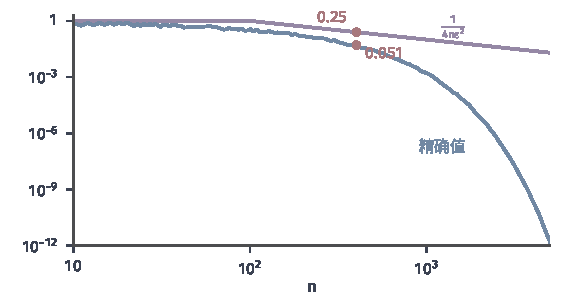
\includegraphics[width=96mm]{figures/07-probability/03-probability-limits/matplotlib/lln-wlln-chebyshev/figure.pdf}
 \caption{均匀硬币的频率偏离$1/2$至少$0.05$的概率，双对数坐标。蓝线为二项分布的精确值，紫线为Chebyshev界$\min\{1,1/(4n\varepsilon^2)\}$，$\varepsilon=0.05$；红点标出$n=400$处的两个值。}
 \label{fig:lln-wlln-chebyshev}
\end{BookInlineFigure}

\paragraph{速度依赖二阶矩}
式~\eqref{eq:lln-wlln-chebyshev}的$1/n$速度来自方差有限这一假设。只知道一阶矩有限时，Chebyshev不等式无法使用，一般也得不到这样的速度：下一小节的Pareto例子中，样本平均的路径时有大的跳跃，靠近均值的过程明显更慢。

\subsection{可积情形}
\label{sec:lln-wlln-integrable}

很多分布均值有限而方差无穷。第~\ref{chap:tail-probabilities}章的Pareto分布，密度为$\alpha x^{-\alpha-1}$（$x\geq1$），取$\alpha=1.5$时
\[
 \mathbb{E}[X]=\int_1^{\infty}x\cdot1.5x^{-2.5}\,\mathrm{d}x=3,\qquad \mathbb{E}[X^2]=\int_1^{\infty}1.5x^{-0.5}\,\mathrm{d}x=\infty .
\]
这时$\operatorname{Var}(\bar{X}_n)=\infty$，Chebyshev不等式无从下手。平均仍应抹平波动，困难在于偶尔出现的大值。办法是先截断：截断后的部分有界，可以用上一小节；被截掉的部分出现得少，用一阶矩控制。

\begin{theorem}[可积情形的弱大数律]
\label{thm:lln-wlln-integrable}
设$X_1,X_2,\dots$独立同分布，$\mathbb{E}[\lvert X_1\rvert]<\infty$，$\mu=\mathbb{E}[X_1]$。则$\bar{X}_n\xrightarrow{\mathbb{P}}\mu$。
\end{theorem}

\begin{proof}
固定$c>0$，把每项分成截断部分与被截掉的部分：
\[
 Y_k=X_k\mathbf{1}_{\{\lvert X_k\rvert\leq c\}},\qquad Z_k=X_k-Y_k=X_k\mathbf{1}_{\{\lvert X_k\rvert>c\}} ,
\]
并记
\[
 \mu_c=\mathbb{E}[Y_1],\qquad \tau(c)=\mathbb{E}\bigl[\lvert X_1\rvert\mathbf{1}_{\{\lvert X_1\rvert>c\}}\bigr]=\mathbb{E}[\lvert Z_1\rvert] .
\]
$\tau(c)$是截掉部分的平均大小。由$\mu=\mu_c+\mathbb{E}[Z_1]$，样本平均的偏差拆成三项：
\[
 \bar{X}_n-\mu=\bigl(\bar{Y}_n-\mu_c\bigr)+\bar{Z}_n-\mathbb{E}[Z_1] ,
\]
其中$\bar{Y}_n$、$\bar{Z}_n$是$Y_k$、$Z_k$的平均。最后一项满足$\lvert\mathbb{E}[Z_1]\rvert\leq\tau(c)$。

固定$\varepsilon>0$，并先假设$c$足够大，使$\tau(c)<\varepsilon/3$。若$\lvert\bar{X}_n-\mu\rvert\geq\varepsilon$，则前两项中至少有一项的绝对值不小于$\varepsilon/3$，所以
\[
 \mathbb{P}\bigl(\lvert\bar{X}_n-\mu\rvert\geq\varepsilon\bigr)\leq\mathbb{P}\bigl(\lvert\bar{Y}_n-\mu_c\rvert\geq\tfrac{\varepsilon}{3}\bigr)+\mathbb{P}\bigl(\lvert\bar{Z}_n\rvert\geq\tfrac{\varepsilon}{3}\bigr) .
\]

第一项是有界变量的平均。$Y_k$独立同分布，且$\lvert Y_1\rvert\leq c$，所以
\[
 \operatorname{Var}(Y_1)\leq\mathbb{E}[Y_1^2]\leq c\,\mathbb{E}[\lvert Y_1\rvert]\leq c\,\mathbb{E}[\lvert X_1\rvert] .
\]
由定理~\ref{thm:lln-wlln-variance}，第一项不超过$9c\,\mathbb{E}[\lvert X_1\rvert]/(n\varepsilon^2)$。第二项用Markov不等式。由三角不等式与同分布，
\[
 \mathbb{E}\bigl[\lvert\bar{Z}_n\rvert\bigr]\leq\frac1n\sum_{k=1}^{n}\mathbb{E}\bigl[\lvert Z_k\rvert\bigr]=\tau(c) ,
\]
所以第二项不超过$3\tau(c)/\varepsilon$。合起来，
\begin{equation}
 \mathbb{P}\bigl(\lvert\bar{X}_n-\mu\rvert\geq\varepsilon\bigr)\leq\frac{9c\,\mathbb{E}[\lvert X_1\rvert]}{n\varepsilon^2}+\frac{3\tau(c)}{\varepsilon} .
 \label{eq:lln-wlln-truncation-bound}
\end{equation}

现在按顺序取极限。先固定$c$令$n\to\infty$，第一项趋于零，得到
\[
 \limsup_{n\to\infty}\mathbb{P}\bigl(\lvert\bar{X}_n-\mu\rvert\geq\varepsilon\bigr)\leq\frac{3\tau(c)}{\varepsilon} .
\]
左边与$c$无关。再令$c\to\infty$：$\lvert X_1\rvert\mathbf{1}_{\{\lvert X_1\rvert>c\}}$逐点趋于零，且被可积的$\lvert X_1\rvert$控制，由支配收敛定理$\tau(c)\to0$。所以左边的上极限为零。
\end{proof}

\paragraph{两个极限的顺序}
式~\eqref{eq:lln-wlln-truncation-bound}的两项此消彼长。截断水平$c$越高，被截掉的部分越小，第二项越小；但留下的部分取值范围越宽，第一项越大。对固定的$n$，令$c\to\infty$会使第一项发散，所以必须先让$n$增大，再放大$c$。等价地说，有用的截断水平要随样本量一起增长，但增长得比$n$慢。

用$\alpha=1.5$的Pareto分布具体看这种权衡。截掉部分的平均大小为
\[
 \tau(c)=\int_c^{\infty}x\cdot1.5x^{-2.5}\,\mathrm{d}x=3c^{-1/2},\qquad c\geq1 ,
\]
截断变量的二阶矩也可以精确算出，
\[
 \mathbb{E}[Y_1^2]=\int_1^c x^2\cdot1.5x^{-2.5}\,\mathrm{d}x=3(\sqrt{c}-1) ,
\]
比证明中用的$c\,\mathbb{E}[X_1]=3c$小得多。取$\varepsilon=1$，用精确的二阶矩代替$c\,\mathbb{E}[\lvert X_1\rvert]$，上界成为
\[
 \frac{27(\sqrt{c}-1)}{n}+\frac{9}{\sqrt{c}},\qquad c>81 ,
\]
其中$c>81$保证$\tau(c)<1/3$。

图~\ref{fig:lln-truncation-tradeoff}(a)画出被截掉的部分：曲线$xf(x)$下$c$右侧的面积就是$\tau(c)$。图(b)画出不同$n$下的总上界。$n=10^4$时最佳截断约为$c\approx3.4\times10^3$，上界约为$0.31$；$n=10^6$时最佳截断移到$c\approx3.3\times10^5$，上界降到约$0.031$。最佳截断水平随$n$增长，上界随之下降。

\begin{BookInlineFigure}
 \centering
 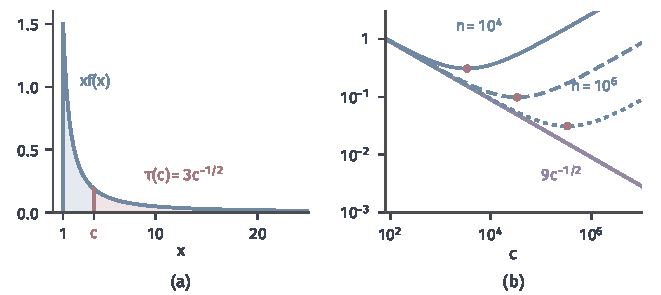
\includegraphics[width=112mm]{figures/07-probability/03-probability-limits/matplotlib/lln-truncation-tradeoff/figure.pdf}
 \caption{$\alpha=1.5$的Pareto分布在弱大数律证明中的截断权衡。(a)求均值的被积函数$xf(x)=1.5x^{-1.5}$（蓝线），截断水平$c=4$左侧为保留部分（浅蓝），右侧为截掉部分（浅红），右侧面积为$\tau(4)=1.5$；(b)$\varepsilon=1$时的上界$27(\sqrt{c}-1)/n+9c^{-1/2}$，蓝色实线、虚线、点线分别对应$n=10^4,10^5,10^6$，红点为各自的最小值，紫线为与$n$无关的第二项$9c^{-1/2}$，双对数坐标。}
 \label{fig:lln-truncation-tradeoff}
\end{BookInlineFigure}

\paragraph{平均意义下的收敛}
同一个截断论证还给出$L^1$收敛。由三角不等式，并对$W=\bar{Y}_n-\mu_c$用一阶绝对矩不超过二阶矩的平方根，
\[
 \mathbb{E}\bigl[\lvert\bar{X}_n-\mu\rvert\bigr]\leq\sqrt{\operatorname{Var}(\bar{Y}_n)}+\mathbb{E}[\lvert\bar{Z}_n\rvert]+\tau(c)\leq\sqrt{\frac{c\,\mathbb{E}[\lvert X_1\rvert]}{n}}+2\tau(c) .
\]
同样先令$n\to\infty$再令$c\to\infty$，得到$\bar{X}_n\xrightarrow{L^{1}}\mu$。

\paragraph{可积不是有限方差}
定理只要求$\mathbb{E}[\lvert X_1\rvert]<\infty$。图~\ref{fig:lln-pareto-cauchy}(a)是$\alpha=1.5$的Pareto样本平均：五条路径最终都靠近$\mu=3$，但不时被一个大观测猛地抬高，再慢慢回落。$n=10^5$时五个平均分别约为$3.00$、$2.98$、$2.97$、$2.97$、$2.92$，多数略低于$3$，因为把平均拉回$3$的正是那些尚未出现的稀有大值。

如果连一阶矩都没有，平均就不再稳定。图(b)是标准Cauchy分布的样本平均，路径不断被新的极端值拉到别处。第~\ref{chap:weak-convergence-of-distributions}章用特征函数可以证明，独立标准Cauchy变量的平均$\bar{X}_n$对每个$n$仍服从标准Cauchy分布，于是
\[
 \mathbb{P}\bigl(\lvert\bar{X}_n\rvert\geq1\bigr)=1-\frac{2}{\pi}\arctan1=\frac12\quad\text{对所有}\ n ,
\]
不趋于零。平均$n$个观测与只看一个观测效果相同，抹平机制完全失效。

\begin{BookInlineFigure}
 \centering
 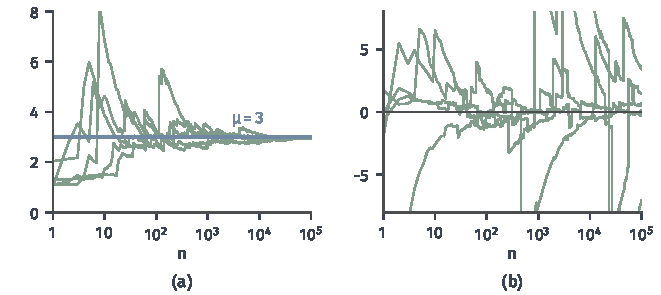
\includegraphics[width=112mm]{figures/07-probability/03-probability-limits/matplotlib/lln-pareto-cauchy/figure.pdf}
 \caption{重尾样本的平均，每图五条路径，横轴为对数刻度。(a)$\alpha=1.5$的Pareto分布（种子$13$），均值$\mu=3$（蓝线），方差无穷；(b)标准Cauchy分布（种子$14$），均值不存在，纵轴截在$[-8,8]$。}
 \label{fig:lln-pareto-cauchy}
\end{BookInlineFigure}


\section{强大数律}
\label{sec:lln-strong-law}

弱大数律对每个固定的$n$说：偏差超过$\varepsilon$的路径只占很小的比例。它没有说同一条路径以后不会再出界。图~\ref{fig:lln-weak-vs-strong}画出$40$条硬币频率路径（种子$21$）与带$0.5\pm0.05$。在$n=400$处只有$3$条在带外，这是弱大数律描述的事情。另一个问题是：沿着一条固定的路径往后看，它是否从某一步起永远留在带内？图中红点标出每条路径在$n\leq2000$内最后一次出带的时刻，最晚的在$n=727$。

\begin{BookInlineFigure}
 \centering
 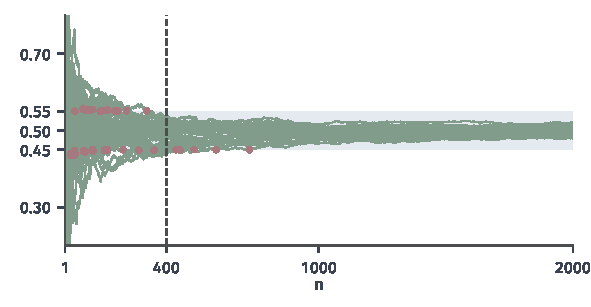
\includegraphics[width=100mm]{figures/07-probability/03-probability-limits/matplotlib/lln-weak-vs-strong/figure.pdf}
 \caption{$40$条均匀硬币的频率路径（绿线，种子$21$），$n\leq2000$。浅蓝带为$0.5\pm0.05$；红点为各路径在图示范围内最后一次位于带外的时刻；虚线标出$n=400$。}
 \label{fig:lln-weak-vs-strong}
\end{BookInlineFigure}

图只能显示有限的范围，“永远留在带内”是关于整条无限路径的断言。把它写成定义，就是几乎必然收敛。

\begin{definition}[强大数律]
\label{def:lln-strong-law}
设随机变量列$X_1,X_2,\dots$各项可积且有共同的均值$\mu$。若$\bar{X}_n\xrightarrow{\mathrm{a.s.}}\mu$，即
\begin{equation}
 \mathbb{P}\Bigl(\lim_{n\to\infty}\bar{X}_n=\mu\Bigr)=1 ,
 \label{eq:lln-strong-law}
\end{equation}
则称这列变量满足\term{强大数律}（strong law of large numbers）。
\end{definition}

由第~\ref{chap:random-variable-convergence}章，几乎必然收敛蕴含依概率收敛，所以强律推出弱律。反过来不能直接升级。Chebyshev界$\sigma^2/(n\varepsilon^2)$对$n$求和发散，Borel–Cantelli引理无从使用：每个时刻出界的概率虽小，加起来却是无穷，不能排除无穷多次出界。要证明强律，需要同时控制所有后续时刻，这正是前两节为随机级数建立的工具。思路是先证明加权级数$\sum_k(X_k-\mu)/k$收敛，再把级数的收敛翻译成平均的收敛。

\subsection{从级数收敛到平均收敛}
\label{sec:lln-series-to-average}

先看一个确定的问题。设实数$x_1,x_2,\dots$使$\sum_kx_k/k$收敛，能否推出$\frac1n\sum_{k\leq n}x_k\to0$？直觉是：级数收敛说明$x_k$按自身大小$k$折算后的累计有限，而前$n$项的总和除以更大的$n$时，早期各项被压小，后期各项又已经很小。

\begin{lemma}[Kronecker引理]
\label{lem:lln-kronecker}
设$0<b_1\leq b_2\leq\cdots$，$b_n\to\infty$，实数列$(x_k)$使$\sum_kx_k/b_k$收敛。则
\begin{equation}
 \lim_{n\to\infty}\frac{1}{b_n}\sum_{k=1}^{n}x_k=0 .
 \label{eq:lln-kronecker}
\end{equation}
\end{lemma}

这个结论称为\term{Kronecker引理}（Kronecker's lemma）。证明用\term{分部求和}（summation by parts），即离散形式的分部积分。

\begin{proof}
记$s_0=0$，$s_n=\sum_{k\leq n}x_k/b_k$，由假设$s_n\to s$。于是$x_k=b_k(s_k-s_{k-1})$。分部求和，把$b_k$与差分$s_k-s_{k-1}$交换位置：
\[
 \sum_{k=1}^{n}x_k=\sum_{k=1}^{n}b_k(s_k-s_{k-1})=b_ns_n-\sum_{k=1}^{n-1}(b_{k+1}-b_k)s_k .
\]
这个恒等式可以按$s_k$的系数逐项核对：$s_n$的系数是$b_n$，$k<n$时$s_k$的系数是$b_k-b_{k+1}$。两边除以$b_n$，
\begin{equation}
 \frac{1}{b_n}\sum_{k=1}^{n}x_k=s_n-\frac{1}{b_n}\sum_{k=1}^{n-1}(b_{k+1}-b_k)s_k .
 \label{eq:lln-abel-identity}
\end{equation}

右边第二项是$s_1,\dots,s_{n-1}$的加权平均，权重$w_{n,k}=(b_{k+1}-b_k)/b_n\geq0$，总和为$(b_n-b_1)/b_n\to1$。下面说明它趋于$s$。给定$\eta>0$，取$N$使$k\geq N$时$\lvert s_k-s\rvert<\eta$。则$n>N$时
\[
 \Bigl\lvert\sum_{k=1}^{n-1}w_{n,k}(s_k-s)\Bigr\rvert\leq\frac{1}{b_n}\sum_{k=1}^{N-1}(b_{k+1}-b_k)\lvert s_k-s\rvert+\eta .
\]
右边第一项的分子与$n$无关，$b_n\to\infty$时趋于零。所以上极限不超过$\eta$，而$\eta$任意。再由$\sum_kw_{n,k}s=s(b_n-b_1)/b_n\to s$，第二项趋于$s$。式~\eqref{eq:lln-abel-identity}的右边趋于$s-s=0$。
\end{proof}

$b_n=n$时，$b_{k+1}-b_k=1$，式~\eqref{eq:lln-abel-identity}的加权平均就是$\frac1n\sum_{k<n}s_k$，即部分和序列的\term{Cesàro平均}（Cesàro mean）。证明的核心是：收敛序列的Cesàro平均收敛到同一极限，而样本平均恰好是原序列与它的Cesàro平均之差。

\paragraph{一个确定的例子}
取$x_k=(-1)^{k+1}\sqrt{k}$。$\sum_kx_k/k=\sum_k(-1)^{k+1}/\sqrt{k}$是交错级数，项的绝对值单调趋于零，所以收敛，和约为$0.6049$。由Kronecker引理，
\[
 \frac1n\sum_{k=1}^{n}(-1)^{k+1}\sqrt{k}\to0 .
\]
直接计算，$n=100,1000,10000$时这个平均分别约为$-0.0463$、$-0.0154$、$-0.0050$，大致与$-1/(2\sqrt{n})$相当。注意$x_k$本身无界，$\lvert x_k\rvert=\sqrt{k}\to\infty$，平均趋于零完全来自正负抵消。

图~\ref{fig:lln-kronecker}画出式~\eqref{eq:lln-abel-identity}中的两项。图(a)中蓝线$s_n$来回振荡地收敛，黄线是它的Cesàro平均，平滑地趋于同一极限；图(b)是二者之差，即样本平均，它被夹在$\pm1/(2\sqrt{n})$之间趋于零。

\begin{BookInlineFigure}
 \centering
 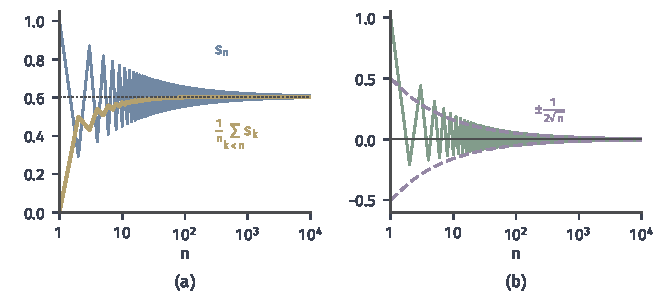
\includegraphics[width=112mm]{figures/07-probability/03-probability-limits/matplotlib/lln-kronecker/figure.pdf}
 \caption{Kronecker引理的恒等式~\eqref{eq:lln-abel-identity}，$b_n=n$，$x_k=(-1)^{k+1}\sqrt{k}$，横轴为对数刻度。(a)$s_n=\sum_{k\leq n}x_k/k$（蓝线）与其Cesàro平均$\frac1n\sum_{k<n}s_k$（黄线），点线为极限$0.6049$；(b)二者之差$\frac1n\sum_{k\leq n}x_k$（绿线）与$\pm1/(2\sqrt{n})$（紫色虚线）。}
 \label{fig:lln-kronecker}
\end{BookInlineFigure}

\paragraph{用到随机变量上}
Kronecker引理是关于实数列的确定性结论。用于随机变量时，先找一个概率为一的事件，在它上面级数收敛，再对其中每个样本点分别使用引理。下面的定理就是这样得到的。

\begin{theorem}[方差加权可和时的强大数律]
\label{thm:lln-kolmogorov-criterion}
设$X_1,X_2,\dots$相互独立，$\mu_k=\mathbb{E}[X_k]$，$\sigma_k^2=\operatorname{Var}(X_k)$，且
\begin{equation}
 \sum_{k=1}^{\infty}\frac{\sigma_k^2}{k^2}<\infty .
 \label{eq:lln-kolmogorov-criterion}
\end{equation}
则
\begin{equation}
 \frac{\tilde{S}_n}{n}=\frac1n\sum_{k=1}^{n}(X_k-\mu_k)\xrightarrow{\mathrm{a.s.}}0 .
 \label{eq:lln-kolmogorov-slln}
\end{equation}
\end{theorem}

\begin{proof}
变量$(X_k-\mu_k)/k$相互独立，均值为零，方差为$\sigma_k^2/k^2$。由条件~\eqref{eq:lln-kolmogorov-criterion}与定理~\ref{thm:lln-variance-series}，存在概率为一的事件$\Omega_0$，在其上级数$\sum_k(X_k-\mu_k)/k$收敛。对每个$\omega\in\Omega_0$，对实数列$x_k=X_k(\omega)-\mu_k$与$b_k=k$用引理~\ref{lem:lln-kronecker}，得到$\tilde{S}_n(\omega)/n\to0$。
\end{proof}

两个特例直接可用。第一，独立同分布且方差$\sigma^2$有限时，$\sum_k\sigma^2/k^2<\infty$，所以$\bar{X}_n\xrightarrow{\mathrm{a.s.}}\mu$：有限方差的强大数律成立。第二，第~\ref{sec:lln-normalization}小节的分段Bernoulli变量满足$\sigma_k^2=p_k(1-p_k)\leq1/4$，条件成立，所以$(S_n-\sum_{k\leq n}p_k)/n\to0$几乎必然成立，这正是图~\ref{fig:lln-varying-means}(b)显示的现象。各项分布不同，样本平均本身却不收敛，强律的正确形式是中心化平均趋于零。

\subsection{独立同分布可积情形}
\label{sec:lln-slln-integrable}

最后去掉有限方差的假设。与弱律一样，办法是截断；不同的是，截断水平这次随项数增长。

\begin{theorem}[强大数律]
\label{thm:lln-slln}
设$X_1,X_2,\dots$独立同分布，$\mathbb{E}[\lvert X_1\rvert]<\infty$，$\mu=\mathbb{E}[X_1]$。则$\bar{X}_n\xrightarrow{\mathrm{a.s.}}\mu$。
\end{theorem}

\begin{proof}
对每个$k$，在水平$k$处截断：
\[
 Y_k=X_k\mathbf{1}_{\{\lvert X_k\rvert\leq k\}} .
\]
$Y_k$是独立变量$X_k$的函数，所以$Y_1,Y_2,\dots$相互独立，但截断水平不同，它们不再同分布。把样本平均的偏差拆成三项：
\[
 \bar{X}_n-\mu=\frac1n\sum_{k=1}^{n}(X_k-Y_k)+\frac1n\sum_{k=1}^{n}\bigl(Y_k-\mathbb{E}[Y_k]\bigr)+\Bigl(\frac1n\sum_{k=1}^{n}\mathbb{E}[Y_k]-\mu\Bigr) .
\]
下面分三步证明每一项几乎必然趋于零。

\emph{第一步：大项只出现有限次。}$X_k$与$X_1$同分布，所以$X_k\neq Y_k$的概率是$\mathbb{P}(\lvert X_1\rvert>k)$。函数$t\mapsto\mathbb{P}(\lvert X_1\rvert>t)$不增，所以它在$t=k$处的值不超过它在区间$[k-1,k]$上的平均：
\[
 \mathbb{P}(\lvert X_1\rvert>k)\leq\int_{k-1}^{k}\mathbb{P}(\lvert X_1\rvert>t)\,\mathrm{d}t .
\]
对$k$求和，再由第~\ref{chap:tail-probabilities}章的尾积分公式，
\[
 \sum_{k=1}^{\infty}\mathbb{P}(\lvert X_1\rvert>k)\leq\int_0^{\infty}\mathbb{P}(\lvert X_1\rvert>t)\,\mathrm{d}t=\mathbb{E}[\lvert X_1\rvert]<\infty .
\]
由Borel–Cantelli引理，几乎必然只有有限个$k$使$X_k\neq Y_k$。在这样的样本点上，$\sum_{k\leq n}(X_k-Y_k)$从某项起不再变化，除以$n$后趋于零。

\emph{第二步：截断均值趋于$\mu$。}由同分布，$\mathbb{E}[Y_k]$等于$X_1\mathbf{1}_{\{\lvert X_1\rvert\leq k\}}$的期望。这个随机变量逐点趋于$X_1$，且被可积的$\lvert X_1\rvert$控制，由支配收敛定理$\mathbb{E}[Y_k]\to\mu$。收敛数列的Cesàro平均收敛到同一极限（这是Kronecker引理证明中的第二步，取$b_n=n$），所以第三项趋于零。

\emph{第三步：截断波动的加权方差可和。}要对$Y_k-\mathbb{E}[Y_k]$用定理~\ref{thm:lln-kolmogorov-criterion}，需检查$\sum_k\operatorname{Var}(Y_k)/k^2<\infty$。由$\operatorname{Var}(Y_k)\leq\mathbb{E}[Y_k^2]$，并交换非负项的求和与期望，
\[
 \sum_{k=1}^{\infty}\frac{\operatorname{Var}(Y_k)}{k^2}\leq\sum_{k=1}^{\infty}\frac{\mathbb{E}\bigl[X_1^2\mathbf{1}_{\{\lvert X_1\rvert\leq k\}}\bigr]}{k^2}=\mathbb{E}\Bigl[X_1^2\sum_{k\geq\lvert X_1\rvert,\,k\geq1}\frac{1}{k^2}\Bigr] .
\]
对实数$x\neq0$，记$m=\lceil\lvert x\rvert\rceil\geq1$，则$m\geq\lvert x\rvert$，并且
\[
 \sum_{k\geq m}\frac{1}{k^2}\leq\frac{1}{m^2}+\int_m^{\infty}\frac{\mathrm{d}t}{t^2}=\frac{1}{m^2}+\frac1m\leq\frac2m\leq\frac{2}{\lvert x\rvert} .
\]
所以期望内的量不超过$x^2\cdot2/\lvert x\rvert=2\lvert x\rvert$；$x=0$时它为零。于是
\[
 \sum_{k=1}^{\infty}\frac{\operatorname{Var}(Y_k)}{k^2}\leq2\,\mathbb{E}[\lvert X_1\rvert]<\infty .
\]
由定理~\ref{thm:lln-kolmogorov-criterion}，第二项几乎必然趋于零。

三项各在一个概率为一的事件上趋于零，三个事件的交概率仍为一，定理得证。
\end{proof}

\paragraph{为什么截断水平取$k$}
若在固定水平$c$截断，被截掉的大值以固定概率$\mathbb{P}(\lvert X_1\rvert>c)>0$反复出现，无穷多次，第一步失效。若截断水平增长得太快，截断变量的方差太大，第三步的级数可能发散。水平$k$恰好使两边都只用到一阶矩：第一步的级数$\sum_k\mathbb{P}(\lvert X_1\rvert>k)$与第三步的级数都被$\mathbb{E}[\lvert X_1\rvert]$控制。

用$\alpha=1.5$的Pareto分布核对两个级数。第一步，$\mathbb{P}(X_1>k)=k^{-1.5}$，
\[
 \sum_{k=1}^{\infty}k^{-1.5}\approx2.612\leq\mathbb{E}[X_1]=3 .
\]
第三步，$\mathbb{E}[Y_k^2]=3(\sqrt{k}-1)$，
\[
 \sum_{k=1}^{\infty}\frac{3(\sqrt{k}-1)}{k^2}\approx2.896\leq2\,\mathbb{E}[X_1]=6 .
\]
图~\ref{fig:lln-truncation-diagonal}画出一组$2000$个Pareto观测（种子$17$）与对角线$x=k$。落在对角线上方、被截断改动的只有$5$个点，位于$k=1,2,10,19,335$；按第一步的级数，期望个数约为$2.57$。$k$越大，越过$k$越难，这些点集中在开头。

\begin{BookInlineFigure}
 \centering
 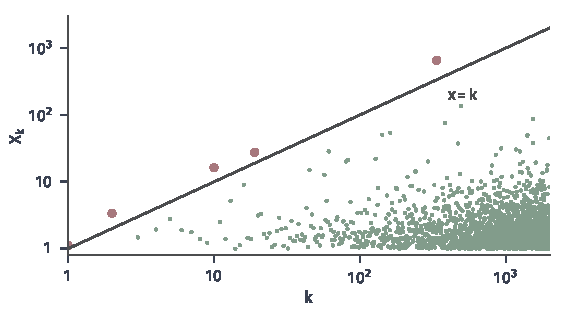
\includegraphics[width=96mm]{figures/07-probability/03-probability-limits/matplotlib/lln-truncation-diagonal/figure.pdf}
 \caption{$\alpha=1.5$的Pareto样本$X_1,\dots,X_{2000}$（种子$17$），双对数坐标。深灰直线为截断水平$x=k$；红点为$X_k>k$、被截断改动的观测，绿点为其余观测。}
 \label{fig:lln-truncation-diagonal}
\end{BookInlineFigure}

\paragraph{可积条件不能去掉}
对独立同分布序列，可积性不仅充分，而且必要。设$\mathbb{E}[\lvert X_1\rvert]=\infty$。与第一步反方向比较，$\mathbb{P}(\lvert X_1\rvert>k)$不小于生存函数在$[k,k+1]$上的平均，所以
\[
 \sum_{k=1}^{\infty}\mathbb{P}(\lvert X_k\rvert>k)\geq\int_1^{\infty}\mathbb{P}(\lvert X_1\rvert>t)\,\mathrm{d}t\geq\mathbb{E}[\lvert X_1\rvert]-1=\infty .
\]
事件$\{\lvert X_k\rvert>k\}$相互独立，由Borel–Cantelli引理的第二部分，几乎必然有无穷多个$k$使$\lvert X_k\rvert/k>1$。另一方面，若$\bar{X}_n$收敛到有限数$L$，则
\[
 \frac{X_n}{n}=\bar{X}_n-\frac{n-1}{n}\bar{X}_{n-1}\to L-L=0 .
\]
两者矛盾，所以$\bar{X}_n$收敛到有限极限的概率为零。图~\ref{fig:lln-pareto-cauchy}(b)的Cauchy路径就是这种情形。

\paragraph{弱律与强律的比较}
表~\ref{tab:lln-weak-strong}把两种大数律放在一起。对独立同分布序列，强律的条件恰好是可积；弱律的结论较弱，它在比可积稍弱的尾部条件下仍可能对适当的中心成立，读者可查阅~\scite{math-kallenberg2021probability}。

\begin{BookInlineTable}
 \centering
 \caption{弱大数律与强大数律（独立同分布，$\mu=\mathbb{E}[X_1]$）。}
 \label{tab:lln-weak-strong}
 \begin{tabular}{lll}
  \toprule
  & 弱大数律 & 强大数律\\
  \midrule
  结论 & 依概率收敛 & 几乎必然收敛\\
  控制对象 & 每个固定时刻 & 整条路径的尾部\\
  有限方差时 & Chebyshev不等式 & 加权级数与Kronecker引理\\
  只有一阶矩时 & 固定水平截断 & 水平随$k$增长的截断\\
  有限样本误差 & 有方差时为$\sigma^2/(n\varepsilon^2)$ & 本身不给速度\\
  \bottomrule
 \end{tabular}
\end{BookInlineTable}

强律回答的是“最终会不会稳定”，它本身不说明何时稳定，也不给出有限样本的误差。对固定的$n$，误差大小仍要靠Chebyshev不等式或更强的集中不等式估计；后者对有界变量给出指数衰减的界，可参考\BookChapterRef{chap:finite-sample-error-bounds}{卷八第4章“有限样本的误差上界”}。


\section{经验平均的应用}
\label{sec:lln-applications}

实际计算中出现的许多量都是平均：一个事件发生的频率、一个函数在观测上的平均、样本的各阶矩。要对它们用大数律，先把它们写成某列随机变量的样本平均，再逐项核对三件事：这列变量是否独立同分布，被平均的函数是否在看到数据之前就已固定，它的期望是否绝对可积。

设$X_1,X_2,\dots$独立同分布，取值于集合$\mathcal{X}$（例如$\mathbb{R}$或$\mathbb{R}^d$），共同分布为$P_X$。本节只讨论预先给定的事件和函数；在看到数据之后再挑选函数或事件，需要对一整族同时成立的保证，那是统计推断的问题。

\subsection{事件频率}
\label{sec:lln-frequency}

第~\ref{chap:classical-probability}章用重复试验中的相对频率解释概率，并在模拟中看到频率稳定在概率附近。现在可以说明它为什么稳定。

对固定的事件$A\subseteq\mathcal{X}$（要求$A$是可测集，即$\{X_1\in A\}$是事件），令
\begin{equation}
 f_n(A)=\frac{1}{n}\sum_{i=1}^{n}\mathbf{1}_{A}(X_i) ,
 \label{eq:lln-frequency}
\end{equation}
即前$n$次观测中落入$A$的比例。示性变量$\mathbf{1}_A(X_i)$独立同分布，服从$\operatorname{Bern}(p)$，其中$p=\mathbb{P}(X_1\in A)$。它们取值于$\{0,1\}$，均值为$p$，方差为$p(1-p)$。

\begin{theorem}[频率的大数律]
\label{thm:lln-frequency}
设$X_1,X_2,\dots$独立同分布，$A$是固定的可测集，$p=\mathbb{P}(X_1\in A)$。则$f_n(A)\xrightarrow{\mathrm{a.s.}}p$，并且对每个$\varepsilon>0$与每个$n$，
\begin{equation}
 \mathbb{P}\bigl(\lvert f_n(A)-p\rvert\geq\varepsilon\bigr)\leq\frac{p(1-p)}{n\varepsilon^2}\leq\frac{1}{4n\varepsilon^2} .
 \label{eq:lln-frequency-bound}
\end{equation}
\end{theorem}

\begin{proof}
示性变量有界，从而可积且方差有限。对它们用定理~\ref{thm:lln-slln}得到几乎必然收敛，用定理~\ref{thm:lln-wlln-variance}得到第一个不等式。第二个不等式来自$p(1-p)\leq1/4$。
\end{proof}

这个结论称为Borel强大数律，它是概率的频率解释的数学内容。以骰子为例，令$A$为“掷出$6$点”，则几乎每一串掷骰记录中$6$点的比例都趋于$1/6$。这里的“几乎每一串”有确切含义：例外的记录（例如永远掷出$6$点）当然可以写下来，但它们的全体概率为零。

\paragraph{随机投点估面积}
频率还可以用来计算面积。设$U,V$独立且都服从$\operatorname{Unif}(0,1)$，事件$A=\{U^2+V^2\leq1\}$是单位正方形中的四分之一圆盘，概率等于它的面积$\pi/4$。在正方形中独立投点，落入圆盘的比例几乎必然趋于$\pi/4$，所以$4f_n(A)\to\pi$。这种用随机样本的平均计算积分的方法称为Monte Carlo方法。

图~\ref{fig:lln-monte-carlo}(a)画出一次投点（种子$31$）的前$400$个点，其中$316$个落在圆内，给出估计$4\times316/400=3.16$。图(b)画出五次独立投点的估计路径，$n=10^4$时它们落在$3.130$到$3.156$之间。式~\eqref{eq:lln-frequency-bound}给出估计的标准差
\[
 4\sqrt{\frac{p(1-p)}{n}}=4\sqrt{\frac{0.7854\times0.2146}{10^4}}\approx0.016 ,
\]
与五个估计的散布相符。误差怎样随样本数缩小、怎样减小它，是第~\ref{chap:monte-carlo-integration-error}章与第~\ref{chap:variance-reduction}章的内容。

\begin{BookInlineFigure}
 \centering
 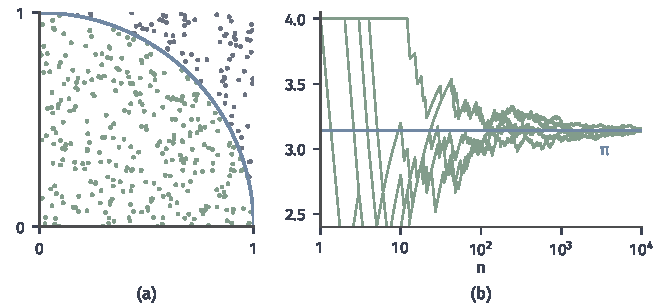
\includegraphics[width=112mm]{figures/07-probability/03-probability-limits/matplotlib/lln-monte-carlo/figure.pdf}
 \caption{用频率估计四分之一圆的面积。(a)单位正方形中的前$400$个均匀点（种子$31$），绿点落在四分之一圆内，灰点落在圆外，蓝线为圆弧；(b)五次独立投点（种子$31$至$35$）的估计$4f_n(A)$（绿线）与$\pi$（蓝线），横轴为对数刻度。}
 \label{fig:lln-monte-carlo}
\end{BookInlineFigure}

\paragraph{固定事件与事件族}
定理~\ref{thm:lln-frequency}对每个固定的$A$给出一个概率为一的事件$\Omega_A$，在其上$f_n(A)\to p$。不同的$A$对应的例外集不同。对可数个事件$A_1,A_2,\dots$，可数个零概率集的并仍是零概率集，所以几乎必然地，$f_n(A_j)\to\mathbb{P}(X_1\in A_j)$对所有$j$同时成立。例如所有端点为有理数的区间可以同时处理。

对所有事件同时成立却是错的。设$X_i$服从$\operatorname{Unif}(0,1)$，取事件$A=\{X_1,\dots,X_n\}$，即观测到的那些点组成的有限集。它的频率是$f_n(A)=1$，概率却是$\mathbb{P}(X_1\in A)=0$，因为连续分布不给单点任何质量。图~\ref{fig:lln-finite-event}画出了这种情形。于是对每个$n$和每个样本点，
\[
 \sup_{A}\bigl\lvert f_n(A)-\mathbb{P}(X_1\in A)\bigr\rvert=1 .
\]

\begin{BookInlineFigure}
 \centering
 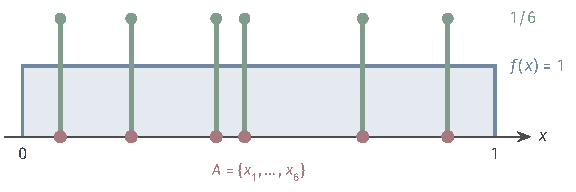
\includegraphics[width=98mm]{figures/07-probability/03-probability-limits/tikz/lln-finite-event/figure.pdf}
 \caption{均匀分布（蓝色，密度为$1$）与六个观测点的经验质量（绿色竖线，每点$1/6$）。由观测点组成的事件$A=\{x_1,\dots,x_6\}$（红点）频率为$1$，在均匀分布下的概率为$0$。}
 \label{fig:lln-finite-event}
\end{BookInlineFigure}

问题出在事件依赖于数据。定理中的$A$必须在观测之前固定。对半直线$(-\infty,t]$这样的特殊事件族，频率可以对整族一致收敛，但那需要额外的论证，属于统计推断的内容，见\BookChapterRef{chap:nonparametric-inference}{卷八第2章“非参数分布与函数推断”}。

\subsection{函数平均与样本矩}
\label{sec:lln-function-averages}

频率是函数平均的特例：被平均的函数是示性函数。一般地，取一个固定的函数$g\colon\mathcal{X}\to\mathbb{R}$（要求可测，使$g(X_1)$是随机变量），考虑$\frac1n\sum_{i\leq n}g(X_i)$。

\begin{theorem}[函数平均的大数律]
\label{thm:lln-function-average}
设$X_1,X_2,\dots$独立同分布，$g$可测，$\mathbb{E}[\lvert g(X_1)\rvert]<\infty$。则
\begin{equation}
 \frac{1}{n}\sum_{i=1}^{n}g(X_i)\xrightarrow{\mathrm{a.s.}}\mathbb{E}[g(X_1)] .
 \label{eq:lln-function-average}
\end{equation}
\end{theorem}

\begin{proof}
$g(X_1),g(X_2),\dots$是独立变量的函数，所以相互独立；它们的分布都是$g(X_1)$的分布，所以同分布。由假设它们可积，对它们用定理~\ref{thm:lln-slln}即可。
\end{proof}

条件$\mathbb{E}[\lvert g(X_1)\rvert]<\infty$必须针对$g(X_1)$检查，而不是针对$X_1$。例如$X_1\sim\operatorname{Unif}(0,1)$有界，但$g(x)=1/x$使
\[
 \mathbb{E}[g(X_1)]=\int_0^1\frac{\mathrm{d}x}{x}=\infty ,
\]
定理不能直接使用。这时平均$\frac1n\sum_i1/X_i$几乎必然趋于$+\infty$：对每个$M>0$，$1/X_i\geq\min\{1/X_i,M\}$，后者有界，由定理得
\[
 \liminf_{n\to\infty}\frac1n\sum_{i=1}^{n}\frac{1}{X_i}\geq\mathbb{E}\bigl[\min\{1/X_1,M\}\bigr]\quad\text{几乎必然},
\]
而右边随$M\to\infty$单调增至$\infty$。取$M=1,2,\dots$，可数个例外集的并仍是零概率集。

\paragraph{样本矩}
取$g(x)=x^r$，$r$为正整数，得到$r$阶\term{样本矩}（sample moment）
\[
 m_{n,r}=\frac{1}{n}\sum_{i=1}^{n}X_i^r .
\]
由定理~\ref{thm:lln-function-average}，只要$\mathbb{E}[\lvert X_1\rvert^r]<\infty$，就有$m_{n,r}\to\mathbb{E}[X_1^r]$几乎必然成立。一阶样本矩就是样本平均$\bar{X}_n$。

\paragraph{样本方差}
常用的\term{样本方差}（sample variance）是
\begin{equation}
 S_n^{2}=\frac{1}{n-1}\sum_{i=1}^{n}\bigl(X_i-\bar{X}_n\bigr)^2,\qquad n\geq2 .
 \label{eq:lln-sample-variance}
\end{equation}
这里$S_n^2$是一个新记号，与部分和$S_n$的平方无关；本小节只在这个意义下使用它。它不是单个函数的平均，因为每一项都含有$\bar{X}_n$。先把平方和展开，用$\sum_iX_i=n\bar{X}_n$，
\[
 \sum_{i=1}^{n}(X_i-\bar{X}_n)^2=\sum_{i=1}^{n}X_i^2-2\bar{X}_n\sum_{i=1}^{n}X_i+n\bar{X}_n^2=\sum_{i=1}^{n}X_i^2-n\bar{X}_n^2 .
\]
于是样本方差写成两个样本矩的组合：
\[
 S_n^{2}=\frac{n}{n-1}\bigl(m_{n,2}-\bar{X}_n^2\bigr) .
\]

现在只需$\mathbb{E}[X_1^2]<\infty$。这时$X_1$也可积，由定理~\ref{thm:lln-function-average}，$m_{n,2}\to\mathbb{E}[X_1^2]$与$\bar{X}_n\to\mu$各在一个概率为一的事件上成立。在两个事件的交上，平方与乘积都是连续运算，$n/(n-1)\to1$，所以
\begin{equation}
 S_n^{2}\xrightarrow{\mathrm{a.s.}}\mathbb{E}[X_1^2]-\mu^2=\sigma^2 .
 \label{eq:lln-sample-variance-limit}
\end{equation}

这个结论只用到有限的二阶矩，不需要假设四阶矩有限。四阶矩控制的是$S_n^2$本身的方差，也就是它在$\sigma^2$附近波动的大小；收敛本身不需要它。

用一组具体数据核对公式。掷五次骰子得到$2,5,3,6,1$，则
\[
 \bar{X}_5=\frac{17}{5}=3.4,\qquad m_{5,2}=\frac{4+25+9+36+1}{5}=15 ,
\]
所以
\[
 S_5^2=\frac54\bigl(15-3.4^2\bigr)=\frac54\times3.44=4.3 .
\]
五次观测太少，$4.3$离$\sigma^2=35/12\approx2.917$还很远。图~\ref{fig:lln-sample-variance}(a)是五条长路径（种子$41$），$n=10^5$时样本方差落在$2.903$到$2.924$之间。

图(b)换成自由度$\nu=3$的t分布（种子$42$）。它的方差为$\nu/(\nu-2)=3$，四阶矩却是无穷。样本方差仍然收敛到$3$，但路径不时被一个大观测猛地推高，再慢慢回落，收敛明显比骰子慢。这正说明四阶矩影响的是波动大小，而不是收敛与否。

\begin{BookInlineFigure}
 \centering
 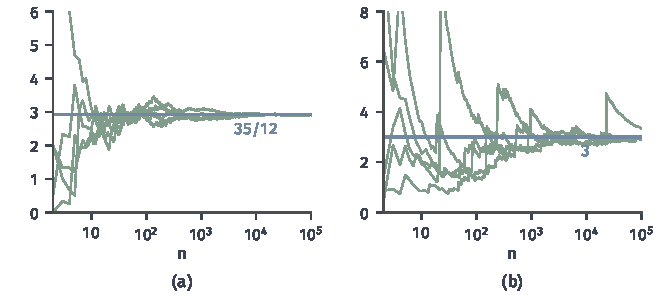
\includegraphics[width=112mm]{figures/07-probability/03-probability-limits/matplotlib/lln-sample-variance/figure.pdf}
 \caption{样本方差$S_n^2$的路径，每图五条（绿线），横轴为对数刻度，蓝线为总体方差。(a)均匀骰子（种子$41$），$\sigma^2=35/12$；(b)自由度$3$的t分布（种子$42$），$\sigma^2=3$，四阶矩无穷。}
 \label{fig:lln-sample-variance}
\end{BookInlineFigure}

\paragraph{适用边界}
本节的结论说明：给定分布与给定函数，经验平均几乎必然趋于相应的期望。它不回答平均以多快的速度接近期望，也不回答在平均附近放大后的误差服从什么分布；前者需要矩或尾部信息，后者是中心极限定理的内容。用样本平均去估计未知的期望、给出可信区间，则是统计推断的问题，由卷八承担。


\section{本章小结}
\label{sec:lln-summary}

本章研究独立随机变量的部分和$S_n$，并区分两个问题：未归一化的累计$\sum_kX_k$是否收敛，以及平均$\bar{X}_n$是否稳定在期望附近。两者用的是同一组工具，各工具解决的环节不同。

\paragraph{部分和的两个基本估计}
独立性使中心化交叉项的期望为零，方差可加，$\operatorname{Var}(S_n)=\sum_k\sigma_k^2$；部分和的散布因此按$\sqrt{n}$增长，样本平均按$1/\sqrt{n}$收窄。Chebyshev不等式只控制固定终点。Kolmogorov最大不等式按首次越过阈值的时刻拆分事件，利用之后增量的独立性与零均值，用同一个终点方差控制整段路径的最大偏离。它需要独立与中心化，两者缺一不可。

\paragraph{随机级数}
最大不等式控制尾段的振荡，于是独立中心化、方差可和的级数几乎必然收敛，同时在$L^2$中收敛。有非零均值时还要单独检查均值级数。方差或均值被罕见大值破坏时，在固定水平截断：大项由超阈值概率可和与Borel–Cantelli引理排除，截断均值由数项级数控制，截断波动由方差可和控制。三系列定理说明这三个条件也是必要的；随机符号级数$\sum_ka_k\varepsilon_k$几乎必然收敛当且仅当$\sum_ka_k^2<\infty$。

\paragraph{两种大数律}
弱大数律回答每个固定时刻偏差的概率。有限方差时Chebyshev不等式给出有限样本的界$\sigma^2/(n\varepsilon^2)$；只有一阶矩时，先固定截断水平、令样本量增大，再放大截断水平。强大数律回答几乎每条路径的最终行为。Kronecker引理把加权级数$\sum_k(X_k-\mu_k)/k$的收敛逐样本地翻译成平均的收敛；对可积的独立同分布序列，按项数$k$截断，使大项只出现有限次、截断方差的加权和被一阶矩控制。可积对强律既充分又必要，Cauchy分布是反例。

\paragraph{使用时核对的条件}
频率、函数平均与样本矩都是独立同分布变量的平均。使用前确认被平均的事件或函数在观测之前固定、相应的期望绝对可积；样本方差的几乎必然收敛只需有限二阶矩。对依赖数据挑选的事件族，单个事件的结论不能直接推广。

大数律确定了平均的极限位置，却没有说明平均在极限附近怎样波动。把偏差$\bar{X}_n-\mu$放大$\sqrt{n}$倍以后，其分布趋于什么形状，需要先建立只比较分布的收敛概念，这是第~\ref{chap:weak-convergence-of-distributions}章与第~\ref{chap:central-limit-theorem}章的内容。

